% DOC SETTINGS ===================================
\documentclass{article}
%%%%%%%%%%%%%%%%%%%%%%%%%%%%%%%%%%%%%%%%%%%%%%%%%%%%%%%%%%%%%%%%%%%%%%%%%%%%%%%% 
%%% ~ Arduino Language - Arduino IDE Colors ~                                  %%%
%%%                                                                            %%%
%%% Kyle Rocha-Brownell | 10/2/2017 | No Licence                               %%%
%%% -------------------------------------------------------------------------- %%%
%%%                                                                            %%%
%%% Place this file in your working directory (next to the latex file you're   %%%
%%% working on).  To add it to your project, place:                            %%%
%%%    %%%%%%%%%%%%%%%%%%%%%%%%%%%%%%%%%%%%%%%%%%%%%%%%%%%%%%%%%%%%%%%%%%%%%%%%%%%%%%%% 
%%% ~ Arduino Language - Arduino IDE Colors ~                                  %%%
%%%                                                                            %%%
%%% Kyle Rocha-Brownell | 10/2/2017 | No Licence                               %%%
%%% -------------------------------------------------------------------------- %%%
%%%                                                                            %%%
%%% Place this file in your working directory (next to the latex file you're   %%%
%%% working on).  To add it to your project, place:                            %%%
%%%    %%%%%%%%%%%%%%%%%%%%%%%%%%%%%%%%%%%%%%%%%%%%%%%%%%%%%%%%%%%%%%%%%%%%%%%%%%%%%%%% 
%%% ~ Arduino Language - Arduino IDE Colors ~                                  %%%
%%%                                                                            %%%
%%% Kyle Rocha-Brownell | 10/2/2017 | No Licence                               %%%
%%% -------------------------------------------------------------------------- %%%
%%%                                                                            %%%
%%% Place this file in your working directory (next to the latex file you're   %%%
%%% working on).  To add it to your project, place:                            %%%
%%%    \input{arduinoLanguage.tex}                                             %%%
%%% somewhere before \begin{document} in your latex file.                      %%%
%%%                                                                            %%%
%%% In your document, place your arduino code between:                         %%%
%%%   \begin{lstlisting}[language=Arduino]                                     %%%
%%% and:                                                                       %%%
%%%   \end{lstlisting}                                                         %%%
%%%                                                                            %%%
%%% Or create your own style to add non-built-in functions and variables.      %%%
%%%                                                                            %%%
 %%%%%%%%%%%%%%%%%%%%%%%%%%%%%%%%%%%%%%%%%%%%%%%%%%%%%%%%%%%%%%%%%%%%%%%%%%%%%%%% 

\usepackage{color}
\usepackage{listings}    
\usepackage{courier}

%%% Define Custom IDE Colors %%%
\definecolor{arduinoGreen}    {rgb} {0.17, 0.43, 0.01}
\definecolor{arduinoGrey}     {rgb} {0.47, 0.47, 0.33}
\definecolor{arduinoOrange}   {rgb} {0.8 , 0.4 , 0   }
\definecolor{arduinoBlue}     {rgb} {0.01, 0.61, 0.98}
\definecolor{arduinoDarkBlue} {rgb} {0.0 , 0.2 , 0.5 }

%%% Define Arduino Language %%%
\lstdefinelanguage{Arduino}{
  language=C++, % begin with default C++ settings 
%
%
  %%% Keyword Color Group 1 %%%  (called KEYWORD3 by arduino)
  keywordstyle=\color{arduinoGreen},   
  deletekeywords={  % remove all arduino keywords that might be in c++
                break, case, override, final, continue, default, do, else, for, 
                if, return, goto, switch, throw, try, while, setup, loop, export, 
                not, or, and, xor, include, define, elif, else, error, if, ifdef, 
                ifndef, pragma, warning,
                HIGH, LOW, INPUT, INPUT_PULLUP, OUTPUT, DEC, BIN, HEX, OCT, PI, 
                HALF_PI, TWO_PI, LSBFIRST, MSBFIRST, CHANGE, FALLING, RISING, 
                DEFAULT, EXTERNAL, INTERNAL, INTERNAL1V1, INTERNAL2V56, LED_BUILTIN, 
                LED_BUILTIN_RX, LED_BUILTIN_TX, DIGITAL_MESSAGE, FIRMATA_STRING, 
                ANALOG_MESSAGE, REPORT_DIGITAL, REPORT_ANALOG, SET_PIN_MODE, 
                SYSTEM_RESET, SYSEX_START, auto, int8_t, int16_t, int32_t, int64_t, 
                uint8_t, uint16_t, uint32_t, uint64_t, char16_t, char32_t, operator, 
                enum, delete, bool, boolean, byte, char, const, false, float, double, 
                null, NULL, int, long, new, private, protected, public, short, 
                signed, static, volatile, String, void, true, unsigned, word, array, 
                sizeof, dynamic_cast, typedef, const_cast, struct, static_cast, union, 
                friend, extern, class, reinterpret_cast, register, explicit, inline, 
                _Bool, complex, _Complex, _Imaginary, atomic_bool, atomic_char, 
                atomic_schar, atomic_uchar, atomic_short, atomic_ushort, atomic_int, 
                atomic_uint, atomic_long, atomic_ulong, atomic_llong, atomic_ullong, 
                virtual, PROGMEM,
                Serial, Serial1, Serial2, Serial3, SerialUSB, Keyboard, Mouse,
                abs, acos, asin, atan, atan2, ceil, constrain, cos, degrees, exp, 
                floor, log, map, max, min, radians, random, randomSeed, round, sin, 
                sq, sqrt, tan, pow, bitRead, bitWrite, bitSet, bitClear, bit, 
                highByte, lowByte, analogReference, analogRead, 
                analogReadResolution, analogWrite, analogWriteResolution, 
                attachInterrupt, detachInterrupt, digitalPinToInterrupt, delay, 
                delayMicroseconds, digitalWrite, digitalRead, interrupts, millis, 
                micros, noInterrupts, noTone, pinMode, pulseIn, pulseInLong, shiftIn, 
                shiftOut, tone, yield, Stream, begin, end, peek, read, print, 
                println, available, availableForWrite, flush, setTimeout, find, 
                findUntil, parseInt, parseFloat, readBytes, readBytesUntil, readString, 
                readStringUntil, trim, toUpperCase, toLowerCase, charAt, compareTo, 
                concat, endsWith, startsWith, equals, equalsIgnoreCase, getBytes, 
                indexOf, lastIndexOf, length, replace, setCharAt, substring, 
                toCharArray, toInt, press, release, releaseAll, accept, click, move, 
                isPressed, isAlphaNumeric, isAlpha, isAscii, isWhitespace, isControl, 
                isDigit, isGraph, isLowerCase, isPrintable, isPunct, isSpace, 
                isUpperCase, isHexadecimalDigit, 
                }, 
  morekeywords={   % add arduino structures to group 1
                break, case, override, final, continue, default, do, else, for, 
                if, return, goto, switch, throw, try, while, setup, loop, export, 
                not, or, and, xor, include, define, elif, else, error, if, ifdef, 
                ifndef, pragma, warning,
                }, 
% 
%
  %%% Keyword Color Group 2 %%%  (called LITERAL1 by arduino)
  keywordstyle=[2]\color{arduinoBlue},   
  keywords=[2]{   % add variables and dataTypes as 2nd group  
                HIGH, LOW, INPUT, INPUT_PULLUP, OUTPUT, DEC, BIN, HEX, OCT, PI, 
                HALF_PI, TWO_PI, LSBFIRST, MSBFIRST, CHANGE, FALLING, RISING, 
                DEFAULT, EXTERNAL, INTERNAL, INTERNAL1V1, INTERNAL2V56, LED_BUILTIN, 
                LED_BUILTIN_RX, LED_BUILTIN_TX, DIGITAL_MESSAGE, FIRMATA_STRING, 
                ANALOG_MESSAGE, REPORT_DIGITAL, REPORT_ANALOG, SET_PIN_MODE, 
                SYSTEM_RESET, SYSEX_START, auto, int8_t, int16_t, int32_t, int64_t, 
                uint8_t, uint16_t, uint32_t, uint64_t, char16_t, char32_t, operator, 
                enum, delete, bool, boolean, byte, char, const, false, float, double, 
                null, NULL, int, long, new, private, protected, public, short, 
                signed, static, volatile, String, void, true, unsigned, word, array, 
                sizeof, dynamic_cast, typedef, const_cast, struct, static_cast, union, 
                friend, extern, class, reinterpret_cast, register, explicit, inline, 
                _Bool, complex, _Complex, _Imaginary, atomic_bool, atomic_char, 
                atomic_schar, atomic_uchar, atomic_short, atomic_ushort, atomic_int, 
                atomic_uint, atomic_long, atomic_ulong, atomic_llong, atomic_ullong, 
                virtual, PROGMEM,
                },  
% 
%
  %%% Keyword Color Group 3 %%%  (called KEYWORD1 by arduino)
  keywordstyle=[3]\bfseries\color{arduinoOrange},
  keywords=[3]{  % add built-in functions as a 3rd group
                Serial, Serial1, Serial2, Serial3, SerialUSB, Keyboard, Mouse,
                },      
%
%
  %%% Keyword Color Group 4 %%%  (called KEYWORD2 by arduino)
  keywordstyle=[4]\color{arduinoOrange},
  keywords=[4]{  % add more built-in functions as a 4th group
                abs, acos, asin, atan, atan2, ceil, constrain, cos, degrees, exp, 
                floor, log, map, max, min, radians, random, randomSeed, round, sin, 
                sq, sqrt, tan, pow, bitRead, bitWrite, bitSet, bitClear, bit, 
                highByte, lowByte, analogReference, analogRead, 
                analogReadResolution, analogWrite, analogWriteResolution, 
                attachInterrupt, detachInterrupt, digitalPinToInterrupt, delay, 
                delayMicroseconds, digitalWrite, digitalRead, interrupts, millis, 
                micros, noInterrupts, noTone, pinMode, pulseIn, pulseInLong, shiftIn, 
                shiftOut, tone, yield, Stream, begin, end, peek, read, print, 
                println, available, availableForWrite, flush, setTimeout, find, 
                findUntil, parseInt, parseFloat, readBytes, readBytesUntil, readString, 
                readStringUntil, trim, toUpperCase, toLowerCase, charAt, compareTo, 
                concat, endsWith, startsWith, equals, equalsIgnoreCase, getBytes, 
                indexOf, lastIndexOf, length, replace, setCharAt, substring, 
                toCharArray, toInt, press, release, releaseAll, accept, click, move, 
                isPressed, isAlphaNumeric, isAlpha, isAscii, isWhitespace, isControl, 
                isDigit, isGraph, isLowerCase, isPrintable, isPunct, isSpace, 
                isUpperCase, isHexadecimalDigit, 
                },      
%
%
  %%% Set Other Colors %%%
  stringstyle=\color{arduinoDarkBlue},    
  commentstyle=\color{arduinoGrey},    
%          
%   
  %%%% Line Numbering %%%%
   numbers=left,                    
  numbersep=5pt,                   
  numberstyle=\color{arduinoGrey},    
  %stepnumber=2,                      % show every 2 line numbers
%
%
  %%%% Code Box Style %%%%
  breaklines=true,                    % wordwrapping
  tabsize=2,         
  basicstyle=\ttfamily  
}                                             %%%
%%% somewhere before \begin{document} in your latex file.                      %%%
%%%                                                                            %%%
%%% In your document, place your arduino code between:                         %%%
%%%   \begin{lstlisting}[language=Arduino]                                     %%%
%%% and:                                                                       %%%
%%%   \end{lstlisting}                                                         %%%
%%%                                                                            %%%
%%% Or create your own style to add non-built-in functions and variables.      %%%
%%%                                                                            %%%
 %%%%%%%%%%%%%%%%%%%%%%%%%%%%%%%%%%%%%%%%%%%%%%%%%%%%%%%%%%%%%%%%%%%%%%%%%%%%%%%% 

\usepackage{color}
\usepackage{listings}    
\usepackage{courier}

%%% Define Custom IDE Colors %%%
\definecolor{arduinoGreen}    {rgb} {0.17, 0.43, 0.01}
\definecolor{arduinoGrey}     {rgb} {0.47, 0.47, 0.33}
\definecolor{arduinoOrange}   {rgb} {0.8 , 0.4 , 0   }
\definecolor{arduinoBlue}     {rgb} {0.01, 0.61, 0.98}
\definecolor{arduinoDarkBlue} {rgb} {0.0 , 0.2 , 0.5 }

%%% Define Arduino Language %%%
\lstdefinelanguage{Arduino}{
  language=C++, % begin with default C++ settings 
%
%
  %%% Keyword Color Group 1 %%%  (called KEYWORD3 by arduino)
  keywordstyle=\color{arduinoGreen},   
  deletekeywords={  % remove all arduino keywords that might be in c++
                break, case, override, final, continue, default, do, else, for, 
                if, return, goto, switch, throw, try, while, setup, loop, export, 
                not, or, and, xor, include, define, elif, else, error, if, ifdef, 
                ifndef, pragma, warning,
                HIGH, LOW, INPUT, INPUT_PULLUP, OUTPUT, DEC, BIN, HEX, OCT, PI, 
                HALF_PI, TWO_PI, LSBFIRST, MSBFIRST, CHANGE, FALLING, RISING, 
                DEFAULT, EXTERNAL, INTERNAL, INTERNAL1V1, INTERNAL2V56, LED_BUILTIN, 
                LED_BUILTIN_RX, LED_BUILTIN_TX, DIGITAL_MESSAGE, FIRMATA_STRING, 
                ANALOG_MESSAGE, REPORT_DIGITAL, REPORT_ANALOG, SET_PIN_MODE, 
                SYSTEM_RESET, SYSEX_START, auto, int8_t, int16_t, int32_t, int64_t, 
                uint8_t, uint16_t, uint32_t, uint64_t, char16_t, char32_t, operator, 
                enum, delete, bool, boolean, byte, char, const, false, float, double, 
                null, NULL, int, long, new, private, protected, public, short, 
                signed, static, volatile, String, void, true, unsigned, word, array, 
                sizeof, dynamic_cast, typedef, const_cast, struct, static_cast, union, 
                friend, extern, class, reinterpret_cast, register, explicit, inline, 
                _Bool, complex, _Complex, _Imaginary, atomic_bool, atomic_char, 
                atomic_schar, atomic_uchar, atomic_short, atomic_ushort, atomic_int, 
                atomic_uint, atomic_long, atomic_ulong, atomic_llong, atomic_ullong, 
                virtual, PROGMEM,
                Serial, Serial1, Serial2, Serial3, SerialUSB, Keyboard, Mouse,
                abs, acos, asin, atan, atan2, ceil, constrain, cos, degrees, exp, 
                floor, log, map, max, min, radians, random, randomSeed, round, sin, 
                sq, sqrt, tan, pow, bitRead, bitWrite, bitSet, bitClear, bit, 
                highByte, lowByte, analogReference, analogRead, 
                analogReadResolution, analogWrite, analogWriteResolution, 
                attachInterrupt, detachInterrupt, digitalPinToInterrupt, delay, 
                delayMicroseconds, digitalWrite, digitalRead, interrupts, millis, 
                micros, noInterrupts, noTone, pinMode, pulseIn, pulseInLong, shiftIn, 
                shiftOut, tone, yield, Stream, begin, end, peek, read, print, 
                println, available, availableForWrite, flush, setTimeout, find, 
                findUntil, parseInt, parseFloat, readBytes, readBytesUntil, readString, 
                readStringUntil, trim, toUpperCase, toLowerCase, charAt, compareTo, 
                concat, endsWith, startsWith, equals, equalsIgnoreCase, getBytes, 
                indexOf, lastIndexOf, length, replace, setCharAt, substring, 
                toCharArray, toInt, press, release, releaseAll, accept, click, move, 
                isPressed, isAlphaNumeric, isAlpha, isAscii, isWhitespace, isControl, 
                isDigit, isGraph, isLowerCase, isPrintable, isPunct, isSpace, 
                isUpperCase, isHexadecimalDigit, 
                }, 
  morekeywords={   % add arduino structures to group 1
                break, case, override, final, continue, default, do, else, for, 
                if, return, goto, switch, throw, try, while, setup, loop, export, 
                not, or, and, xor, include, define, elif, else, error, if, ifdef, 
                ifndef, pragma, warning,
                }, 
% 
%
  %%% Keyword Color Group 2 %%%  (called LITERAL1 by arduino)
  keywordstyle=[2]\color{arduinoBlue},   
  keywords=[2]{   % add variables and dataTypes as 2nd group  
                HIGH, LOW, INPUT, INPUT_PULLUP, OUTPUT, DEC, BIN, HEX, OCT, PI, 
                HALF_PI, TWO_PI, LSBFIRST, MSBFIRST, CHANGE, FALLING, RISING, 
                DEFAULT, EXTERNAL, INTERNAL, INTERNAL1V1, INTERNAL2V56, LED_BUILTIN, 
                LED_BUILTIN_RX, LED_BUILTIN_TX, DIGITAL_MESSAGE, FIRMATA_STRING, 
                ANALOG_MESSAGE, REPORT_DIGITAL, REPORT_ANALOG, SET_PIN_MODE, 
                SYSTEM_RESET, SYSEX_START, auto, int8_t, int16_t, int32_t, int64_t, 
                uint8_t, uint16_t, uint32_t, uint64_t, char16_t, char32_t, operator, 
                enum, delete, bool, boolean, byte, char, const, false, float, double, 
                null, NULL, int, long, new, private, protected, public, short, 
                signed, static, volatile, String, void, true, unsigned, word, array, 
                sizeof, dynamic_cast, typedef, const_cast, struct, static_cast, union, 
                friend, extern, class, reinterpret_cast, register, explicit, inline, 
                _Bool, complex, _Complex, _Imaginary, atomic_bool, atomic_char, 
                atomic_schar, atomic_uchar, atomic_short, atomic_ushort, atomic_int, 
                atomic_uint, atomic_long, atomic_ulong, atomic_llong, atomic_ullong, 
                virtual, PROGMEM,
                },  
% 
%
  %%% Keyword Color Group 3 %%%  (called KEYWORD1 by arduino)
  keywordstyle=[3]\bfseries\color{arduinoOrange},
  keywords=[3]{  % add built-in functions as a 3rd group
                Serial, Serial1, Serial2, Serial3, SerialUSB, Keyboard, Mouse,
                },      
%
%
  %%% Keyword Color Group 4 %%%  (called KEYWORD2 by arduino)
  keywordstyle=[4]\color{arduinoOrange},
  keywords=[4]{  % add more built-in functions as a 4th group
                abs, acos, asin, atan, atan2, ceil, constrain, cos, degrees, exp, 
                floor, log, map, max, min, radians, random, randomSeed, round, sin, 
                sq, sqrt, tan, pow, bitRead, bitWrite, bitSet, bitClear, bit, 
                highByte, lowByte, analogReference, analogRead, 
                analogReadResolution, analogWrite, analogWriteResolution, 
                attachInterrupt, detachInterrupt, digitalPinToInterrupt, delay, 
                delayMicroseconds, digitalWrite, digitalRead, interrupts, millis, 
                micros, noInterrupts, noTone, pinMode, pulseIn, pulseInLong, shiftIn, 
                shiftOut, tone, yield, Stream, begin, end, peek, read, print, 
                println, available, availableForWrite, flush, setTimeout, find, 
                findUntil, parseInt, parseFloat, readBytes, readBytesUntil, readString, 
                readStringUntil, trim, toUpperCase, toLowerCase, charAt, compareTo, 
                concat, endsWith, startsWith, equals, equalsIgnoreCase, getBytes, 
                indexOf, lastIndexOf, length, replace, setCharAt, substring, 
                toCharArray, toInt, press, release, releaseAll, accept, click, move, 
                isPressed, isAlphaNumeric, isAlpha, isAscii, isWhitespace, isControl, 
                isDigit, isGraph, isLowerCase, isPrintable, isPunct, isSpace, 
                isUpperCase, isHexadecimalDigit, 
                },      
%
%
  %%% Set Other Colors %%%
  stringstyle=\color{arduinoDarkBlue},    
  commentstyle=\color{arduinoGrey},    
%          
%   
  %%%% Line Numbering %%%%
   numbers=left,                    
  numbersep=5pt,                   
  numberstyle=\color{arduinoGrey},    
  %stepnumber=2,                      % show every 2 line numbers
%
%
  %%%% Code Box Style %%%%
  breaklines=true,                    % wordwrapping
  tabsize=2,         
  basicstyle=\ttfamily  
}                                             %%%
%%% somewhere before \begin{document} in your latex file.                      %%%
%%%                                                                            %%%
%%% In your document, place your arduino code between:                         %%%
%%%   \begin{lstlisting}[language=Arduino]                                     %%%
%%% and:                                                                       %%%
%%%   \end{lstlisting}                                                         %%%
%%%                                                                            %%%
%%% Or create your own style to add non-built-in functions and variables.      %%%
%%%                                                                            %%%
 %%%%%%%%%%%%%%%%%%%%%%%%%%%%%%%%%%%%%%%%%%%%%%%%%%%%%%%%%%%%%%%%%%%%%%%%%%%%%%%% 

\usepackage{color}
\usepackage{listings}    
\usepackage{courier}

%%% Define Custom IDE Colors %%%
\definecolor{arduinoGreen}    {rgb} {0.17, 0.43, 0.01}
\definecolor{arduinoGrey}     {rgb} {0.47, 0.47, 0.33}
\definecolor{arduinoOrange}   {rgb} {0.8 , 0.4 , 0   }
\definecolor{arduinoBlue}     {rgb} {0.01, 0.61, 0.98}
\definecolor{arduinoDarkBlue} {rgb} {0.0 , 0.2 , 0.5 }

%%% Define Arduino Language %%%
\lstdefinelanguage{Arduino}{
  language=C++, % begin with default C++ settings 
%
%
  %%% Keyword Color Group 1 %%%  (called KEYWORD3 by arduino)
  keywordstyle=\color{arduinoGreen},   
  deletekeywords={  % remove all arduino keywords that might be in c++
                break, case, override, final, continue, default, do, else, for, 
                if, return, goto, switch, throw, try, while, setup, loop, export, 
                not, or, and, xor, include, define, elif, else, error, if, ifdef, 
                ifndef, pragma, warning,
                HIGH, LOW, INPUT, INPUT_PULLUP, OUTPUT, DEC, BIN, HEX, OCT, PI, 
                HALF_PI, TWO_PI, LSBFIRST, MSBFIRST, CHANGE, FALLING, RISING, 
                DEFAULT, EXTERNAL, INTERNAL, INTERNAL1V1, INTERNAL2V56, LED_BUILTIN, 
                LED_BUILTIN_RX, LED_BUILTIN_TX, DIGITAL_MESSAGE, FIRMATA_STRING, 
                ANALOG_MESSAGE, REPORT_DIGITAL, REPORT_ANALOG, SET_PIN_MODE, 
                SYSTEM_RESET, SYSEX_START, auto, int8_t, int16_t, int32_t, int64_t, 
                uint8_t, uint16_t, uint32_t, uint64_t, char16_t, char32_t, operator, 
                enum, delete, bool, boolean, byte, char, const, false, float, double, 
                null, NULL, int, long, new, private, protected, public, short, 
                signed, static, volatile, String, void, true, unsigned, word, array, 
                sizeof, dynamic_cast, typedef, const_cast, struct, static_cast, union, 
                friend, extern, class, reinterpret_cast, register, explicit, inline, 
                _Bool, complex, _Complex, _Imaginary, atomic_bool, atomic_char, 
                atomic_schar, atomic_uchar, atomic_short, atomic_ushort, atomic_int, 
                atomic_uint, atomic_long, atomic_ulong, atomic_llong, atomic_ullong, 
                virtual, PROGMEM,
                Serial, Serial1, Serial2, Serial3, SerialUSB, Keyboard, Mouse,
                abs, acos, asin, atan, atan2, ceil, constrain, cos, degrees, exp, 
                floor, log, map, max, min, radians, random, randomSeed, round, sin, 
                sq, sqrt, tan, pow, bitRead, bitWrite, bitSet, bitClear, bit, 
                highByte, lowByte, analogReference, analogRead, 
                analogReadResolution, analogWrite, analogWriteResolution, 
                attachInterrupt, detachInterrupt, digitalPinToInterrupt, delay, 
                delayMicroseconds, digitalWrite, digitalRead, interrupts, millis, 
                micros, noInterrupts, noTone, pinMode, pulseIn, pulseInLong, shiftIn, 
                shiftOut, tone, yield, Stream, begin, end, peek, read, print, 
                println, available, availableForWrite, flush, setTimeout, find, 
                findUntil, parseInt, parseFloat, readBytes, readBytesUntil, readString, 
                readStringUntil, trim, toUpperCase, toLowerCase, charAt, compareTo, 
                concat, endsWith, startsWith, equals, equalsIgnoreCase, getBytes, 
                indexOf, lastIndexOf, length, replace, setCharAt, substring, 
                toCharArray, toInt, press, release, releaseAll, accept, click, move, 
                isPressed, isAlphaNumeric, isAlpha, isAscii, isWhitespace, isControl, 
                isDigit, isGraph, isLowerCase, isPrintable, isPunct, isSpace, 
                isUpperCase, isHexadecimalDigit, 
                }, 
  morekeywords={   % add arduino structures to group 1
                break, case, override, final, continue, default, do, else, for, 
                if, return, goto, switch, throw, try, while, setup, loop, export, 
                not, or, and, xor, include, define, elif, else, error, if, ifdef, 
                ifndef, pragma, warning,
                }, 
% 
%
  %%% Keyword Color Group 2 %%%  (called LITERAL1 by arduino)
  keywordstyle=[2]\color{arduinoBlue},   
  keywords=[2]{   % add variables and dataTypes as 2nd group  
                HIGH, LOW, INPUT, INPUT_PULLUP, OUTPUT, DEC, BIN, HEX, OCT, PI, 
                HALF_PI, TWO_PI, LSBFIRST, MSBFIRST, CHANGE, FALLING, RISING, 
                DEFAULT, EXTERNAL, INTERNAL, INTERNAL1V1, INTERNAL2V56, LED_BUILTIN, 
                LED_BUILTIN_RX, LED_BUILTIN_TX, DIGITAL_MESSAGE, FIRMATA_STRING, 
                ANALOG_MESSAGE, REPORT_DIGITAL, REPORT_ANALOG, SET_PIN_MODE, 
                SYSTEM_RESET, SYSEX_START, auto, int8_t, int16_t, int32_t, int64_t, 
                uint8_t, uint16_t, uint32_t, uint64_t, char16_t, char32_t, operator, 
                enum, delete, bool, boolean, byte, char, const, false, float, double, 
                null, NULL, int, long, new, private, protected, public, short, 
                signed, static, volatile, String, void, true, unsigned, word, array, 
                sizeof, dynamic_cast, typedef, const_cast, struct, static_cast, union, 
                friend, extern, class, reinterpret_cast, register, explicit, inline, 
                _Bool, complex, _Complex, _Imaginary, atomic_bool, atomic_char, 
                atomic_schar, atomic_uchar, atomic_short, atomic_ushort, atomic_int, 
                atomic_uint, atomic_long, atomic_ulong, atomic_llong, atomic_ullong, 
                virtual, PROGMEM,
                },  
% 
%
  %%% Keyword Color Group 3 %%%  (called KEYWORD1 by arduino)
  keywordstyle=[3]\bfseries\color{arduinoOrange},
  keywords=[3]{  % add built-in functions as a 3rd group
                Serial, Serial1, Serial2, Serial3, SerialUSB, Keyboard, Mouse,
                },      
%
%
  %%% Keyword Color Group 4 %%%  (called KEYWORD2 by arduino)
  keywordstyle=[4]\color{arduinoOrange},
  keywords=[4]{  % add more built-in functions as a 4th group
                abs, acos, asin, atan, atan2, ceil, constrain, cos, degrees, exp, 
                floor, log, map, max, min, radians, random, randomSeed, round, sin, 
                sq, sqrt, tan, pow, bitRead, bitWrite, bitSet, bitClear, bit, 
                highByte, lowByte, analogReference, analogRead, 
                analogReadResolution, analogWrite, analogWriteResolution, 
                attachInterrupt, detachInterrupt, digitalPinToInterrupt, delay, 
                delayMicroseconds, digitalWrite, digitalRead, interrupts, millis, 
                micros, noInterrupts, noTone, pinMode, pulseIn, pulseInLong, shiftIn, 
                shiftOut, tone, yield, Stream, begin, end, peek, read, print, 
                println, available, availableForWrite, flush, setTimeout, find, 
                findUntil, parseInt, parseFloat, readBytes, readBytesUntil, readString, 
                readStringUntil, trim, toUpperCase, toLowerCase, charAt, compareTo, 
                concat, endsWith, startsWith, equals, equalsIgnoreCase, getBytes, 
                indexOf, lastIndexOf, length, replace, setCharAt, substring, 
                toCharArray, toInt, press, release, releaseAll, accept, click, move, 
                isPressed, isAlphaNumeric, isAlpha, isAscii, isWhitespace, isControl, 
                isDigit, isGraph, isLowerCase, isPrintable, isPunct, isSpace, 
                isUpperCase, isHexadecimalDigit, 
                },      
%
%
  %%% Set Other Colors %%%
  stringstyle=\color{arduinoDarkBlue},    
  commentstyle=\color{arduinoGrey},    
%          
%   
  %%%% Line Numbering %%%%
   numbers=left,                    
  numbersep=5pt,                   
  numberstyle=\color{arduinoGrey},    
  %stepnumber=2,                      % show every 2 line numbers
%
%
  %%%% Code Box Style %%%%
  breaklines=true,                    % wordwrapping
  tabsize=2,         
  basicstyle=\ttfamily  
}
\usepackage{steinmetz}
\usepackage{mathtools}  
\usepackage{multicol}
\usepackage{circuitikz}
\usepackage{tikz}
\usepackage{listings}
\usepackage{geometry}
\usepackage{fancyhdr}
\usepackage{amsfonts}
\usepackage{media9}
\usepackage{parskip}
\usetikzlibrary{positioning, fit, calc}
\pagestyle{fancy}
\lhead{ECE2804 Lab Journal}
\rhead{Kavin Thirukonda 2021}
\usepackage{hyperref}
\hypersetup{
    colorlinks=true,
    linkcolor=blue,
    filecolor=magenta,      
    urlcolor=cyan,
}
\fancyheadoffset{0mm}
 \geometry{
 a4paper,
 total={170mm,257mm},
 left=20mm,
 top=25mm,
 }
 \usepackage{listings}
\definecolor{codegreen}{rgb}{0,0.6,0}
\definecolor{codegray}{rgb}{0.5,0.5,0.5}
\definecolor{codepurple}{rgb}{0.58,0,0.82}
\definecolor{backcolour}{rgb}{0.95,0.95,0.92}
\lstdefinestyle{codelisting}{
    backgroundcolor=\color{backcolour},   
    commentstyle=\color{codegreen},
    keywordstyle=\color{magenta},
    numberstyle=\tiny\color{codegray},
    stringstyle=\color{codepurple},
    basicstyle=\ttfamily\footnotesize,
    breakatwhitespace=false,         
    breaklines=true,                 
    captionpos=b,                    
    keepspaces=true,                 
    numbers=left,                    
    numbersep=5pt,                  
    showspaces=false,                
    showstringspaces=false,
    showtabs=false,                  
    tabsize=2,
}
\lstset{style=codelisting}
\mathtoolsset{showonlyrefs} 

\usepackage[utf8]{inputenc}
% DOC SETTINGS ===================================
\begin{document}
\maketitle
\newpage
\tableofcontents
\newpage
\section{Introduction}
This project given is the SpO2 project and the project consists of taking a signal from the given Nellcor Ds-100A compatible SpO2 finger sensor. The signal consists of a small AC current signal on top of a larger DC current signal. The signal needs to be amplified, filtered, and amplified again to get the final signal to process into heart rate and SpO2 information. The process starts from early on in the SpO2 sensor where the red and infrared LEDs are pulsed rapidly resulting in an almost continuous signal consisting of the 2 values. The signal then will be inputted into the Arduino where heart rate and SpO2 values will be calculated. The biggest challenge in doing the digital computations is trying to figure out where the peaks are, once the peaks are found everything else gets significantly easier, from there the R ratio can be calculated and the periodic time between the peaks can be found to calculate heart rate.


\section{Block Diagram}
\begin{figure}[h]
    \centering
    \boxed{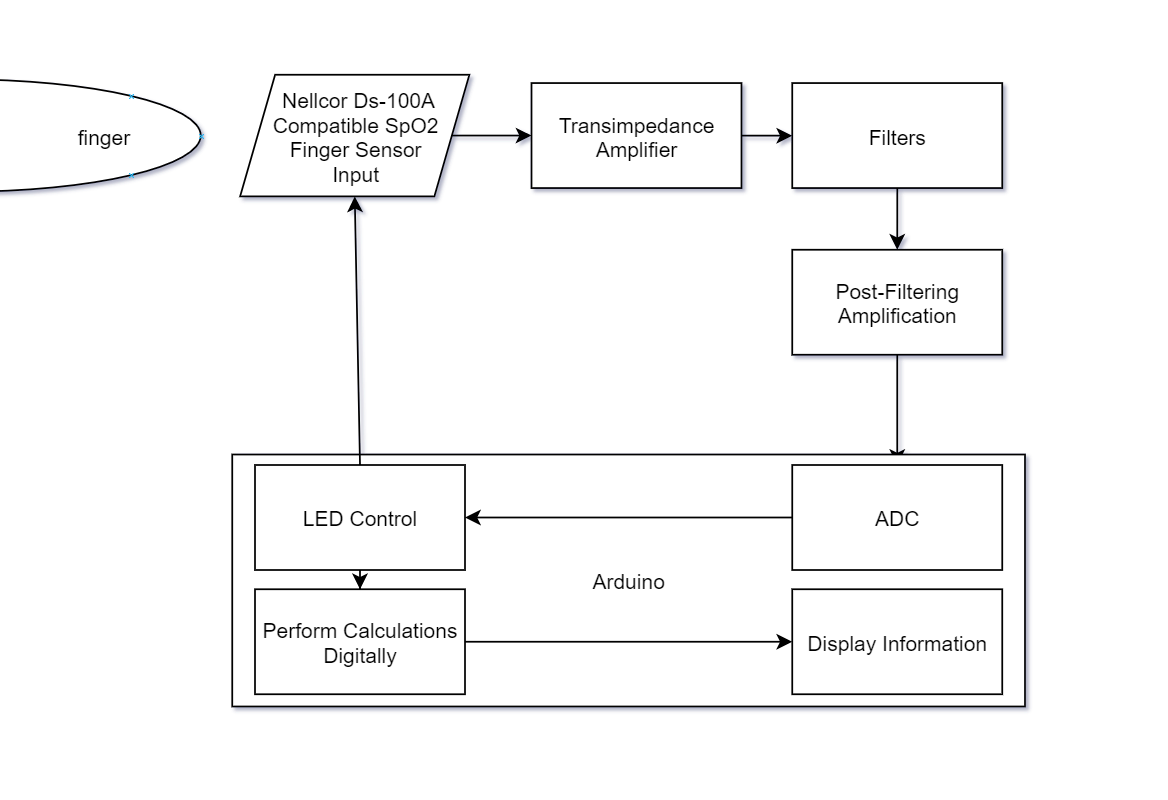
\includegraphics[width = .85\textwidth]{images/blockdiagram.png}}
    \caption{The Block Diagram Containing the Major Parts of the Project}
    \label{figure:BlockDiagram}
\end{figure}

This diagram shows the main components of the circuit, and by designing all of these parts separately you can easily put them together to make the circuit work. Since the narrative of this project is to create a prototype board in preparation for a more compact version later, the next challenge would be to take these blocks and try to fulfill their requirements while still making them as compact as possible such that a consumer would not mind carrying one around if needed.
\newpage
\section{SpO2 Sensor}
It is known that two LEDs in the run anti-parallel to each other thus to turn one them on, one pin on the breakout board pin 5 or pin 6 must be connected to ground and one to +5V. Though there is a limit of current that can be inputted to the LEDs so that the LEDs are not damaged and that was given to be 15mA. This is the max limit but there is also another limit that was found to be the output from the SpO2 sensor at 15mA would be too strong of a signal based on the persons' skin color, thus causing the signal as it is amplified to get "overloaded" becoming a DC signal. This was adjusted with by changing the current entering the LED's and it was found that 6-8mA was a good mid point with the final resistor value being used to be $820\Omega$. Which was found simply by: V = I X R $\rightarrow$ 5V = I X ($820\Omega$) $\rightarrow$ I = 6.09mA.

\section{Switching}
For the ability to calculate the SpO2 levels there must be a ratio of the two signals RED and IRED, the way this needed to be done is by switching between them back and forth fast enough such that the final signal can be seen as continuous to the Arduino by giving it enough data points. The reason they can't be on at the same time is because for one the LEDs are anti parallel and therefore can only be on one at a time. The reason they are configured like this is because having them both on at the same time would cause interference between the lights and the sensor would end up picking up a sort of mix from both the signals instead of a single signal which would be just about as useless as just having one signal since heart rate would only be able to calculated. So by having the LEDs anti parallel they are forced to only stay on one at a time.

Instead of using a timer on the outside to switch between the two LED's rapidly, it was decided that the Arduino would control the LED's, this way there would have to be any type of syncing between the timer making the LED's turn on and off with the code, rather the code would be controlling this and would automatically be synced that way.

This would be implemented by connecting two digital write pins to the $820\Omega$ resistor, which with code the Arduino could toggle back and forth as seen in the code below.
\begin{lstlisting}[language=Arduino, caption= Flashing Code]
//turn off Infrared LED and turn on RED LED
digitalWrite(REDLedPin,HIGH);
digitalWrite(IRLedPin,LOW);
// set counter variable to zero
n = 0;
//record start time
start = millis();
//reset sum variable
scanner = 0.0;
//record values until you reach the end of the MEASURING_PERIOD
do{
  scanner += analogRead (sensorPin);
  n++;
}
while (millis() < start + MEASURING_PERIOD);  
//calculate average
scanner /= n; 
//turn on Infrared LED and turn off RED LED
digitalWrite(REDLedPin,LOW);
digitalWrite(IRLedPin,HIGH);
n = 0;
start = millis();
scanner = 0.0;
do{
  scanner += analogRead (sensorPin);
  n++;
}
while (millis() < start + MEASURING_PERIOD);  
//calculate average
scanner /= n; 
\end{lstlisting}
\newpage


\section{Pre-Filtering Amplification}
After the current signal is output from the SpO2 sensor it can be seen that the signal is a current signal of a magnitude of $1-2\mu$A(depending on finger positioning) which can be seen here when taking a measurement of the signal:
\begin{figure}[h]
    \centering
    \boxed{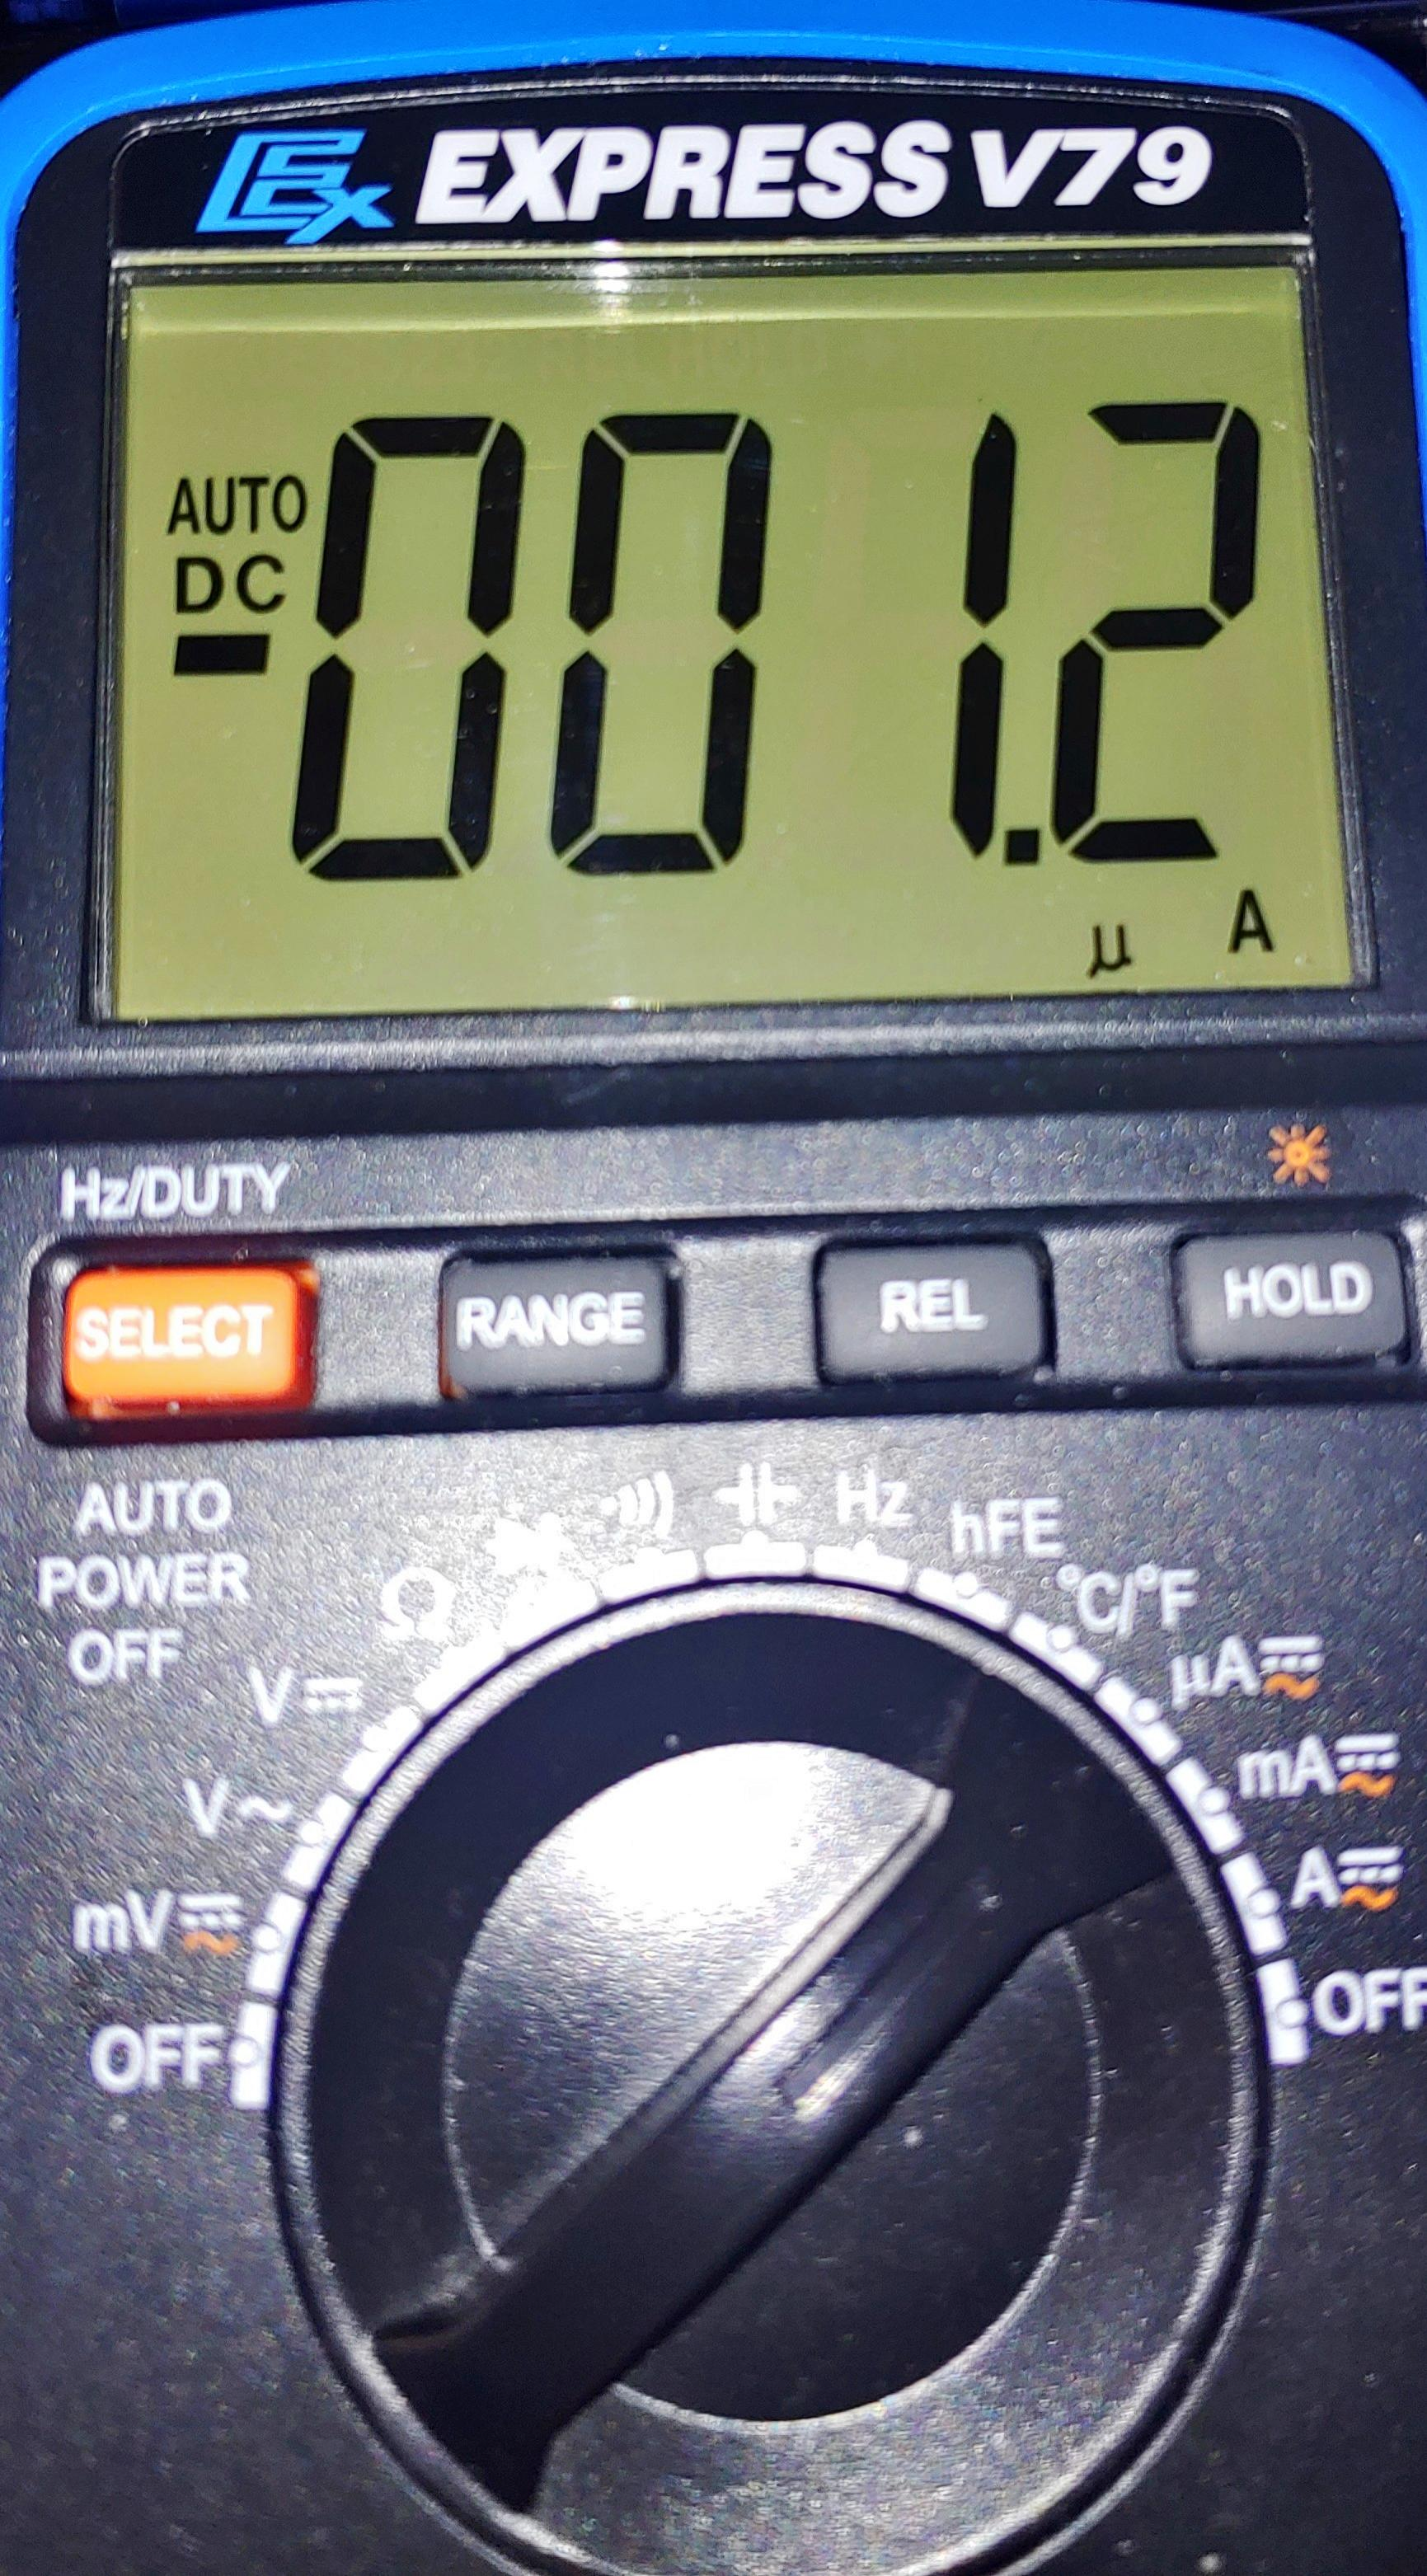
\includegraphics[width = .375\textwidth, height = .475\textwidth]{images/SpO2_O.jpg}}
    \caption{Current Output from the SpO2 Sensor}
    \label{figure:SpO2CurrentOut}
\end{figure}

This means the signal needs to be converted to a voltage signal and amplified, which is achieved by the current to voltage converter circuit. The circuit is determined by the equations of with following results:
\begin{equation}
     V_{out} = -I_{out}*R_{1}
\end{equation}
\begin{equation}
    V_{out} = (1.2\mu A)*(2M\Omega)
\end{equation}
\begin{equation}
    V_{out} = 2.4V
\end{equation}
The calculations results in the final circuit created in LTSpice as seen below:
\begin{figure}[h]
    \centering
    \boxed{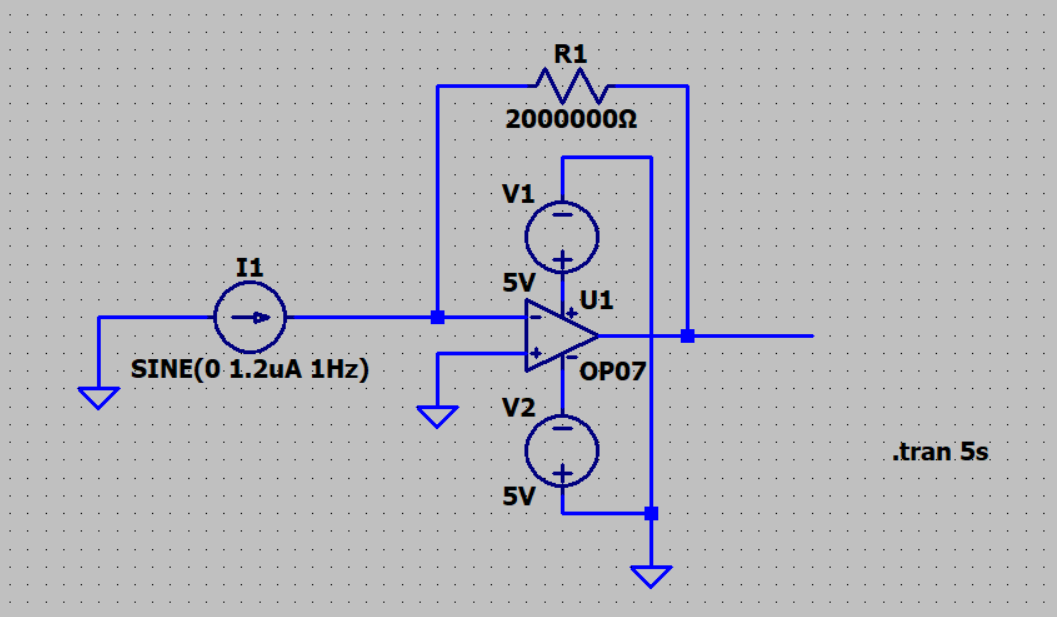
\includegraphics[width = \textwidth, height = .5\textwidth]{images/C_to_V_LT.png}}
    \caption{Current to Voltage Converter LTSpice Schematic}
    \label{figure:CtoVLTSpice}
\end{figure}
\newpage
The results from the simulation of the circuit with a simulated input in LTSpice was:
\begin{figure}[h]
    \centering
    \boxed{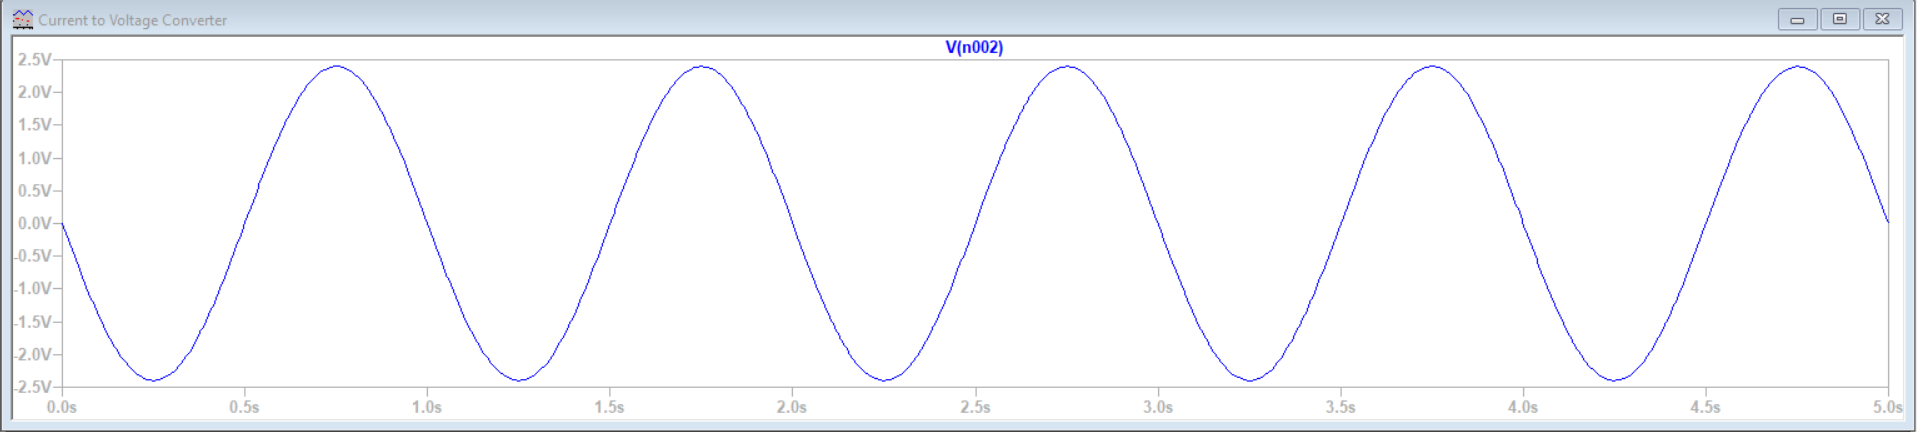
\includegraphics[width = \textwidth]{images/C_to_V_LT_R.png}}
    \caption{Current to Voltage Converter LTSpice Simulation Output}
    \label{figure:CtoVLTSpice_O}
\end{figure}

The circuit achieves this result by the input being a current signal and by the known knowledge that the current input to the op-amp is 0A, thus the current flows through the $2M\Omega$ resistor. This converts the current signal to a voltage signal of around 2V but since both sides of the resistor need to be equivalent to each other, the op-amp will output it's own negative voltage to counteract the voltage from the current signal through the resistor. Therefore resulting the in the negative voltage output from the circuit overall due to the previously explained flow of current and voltage.

When the final circuit is built and connect to the rest of the full circuit it is seen as below:
\begin{figure}[h]
    \centering
    \boxed{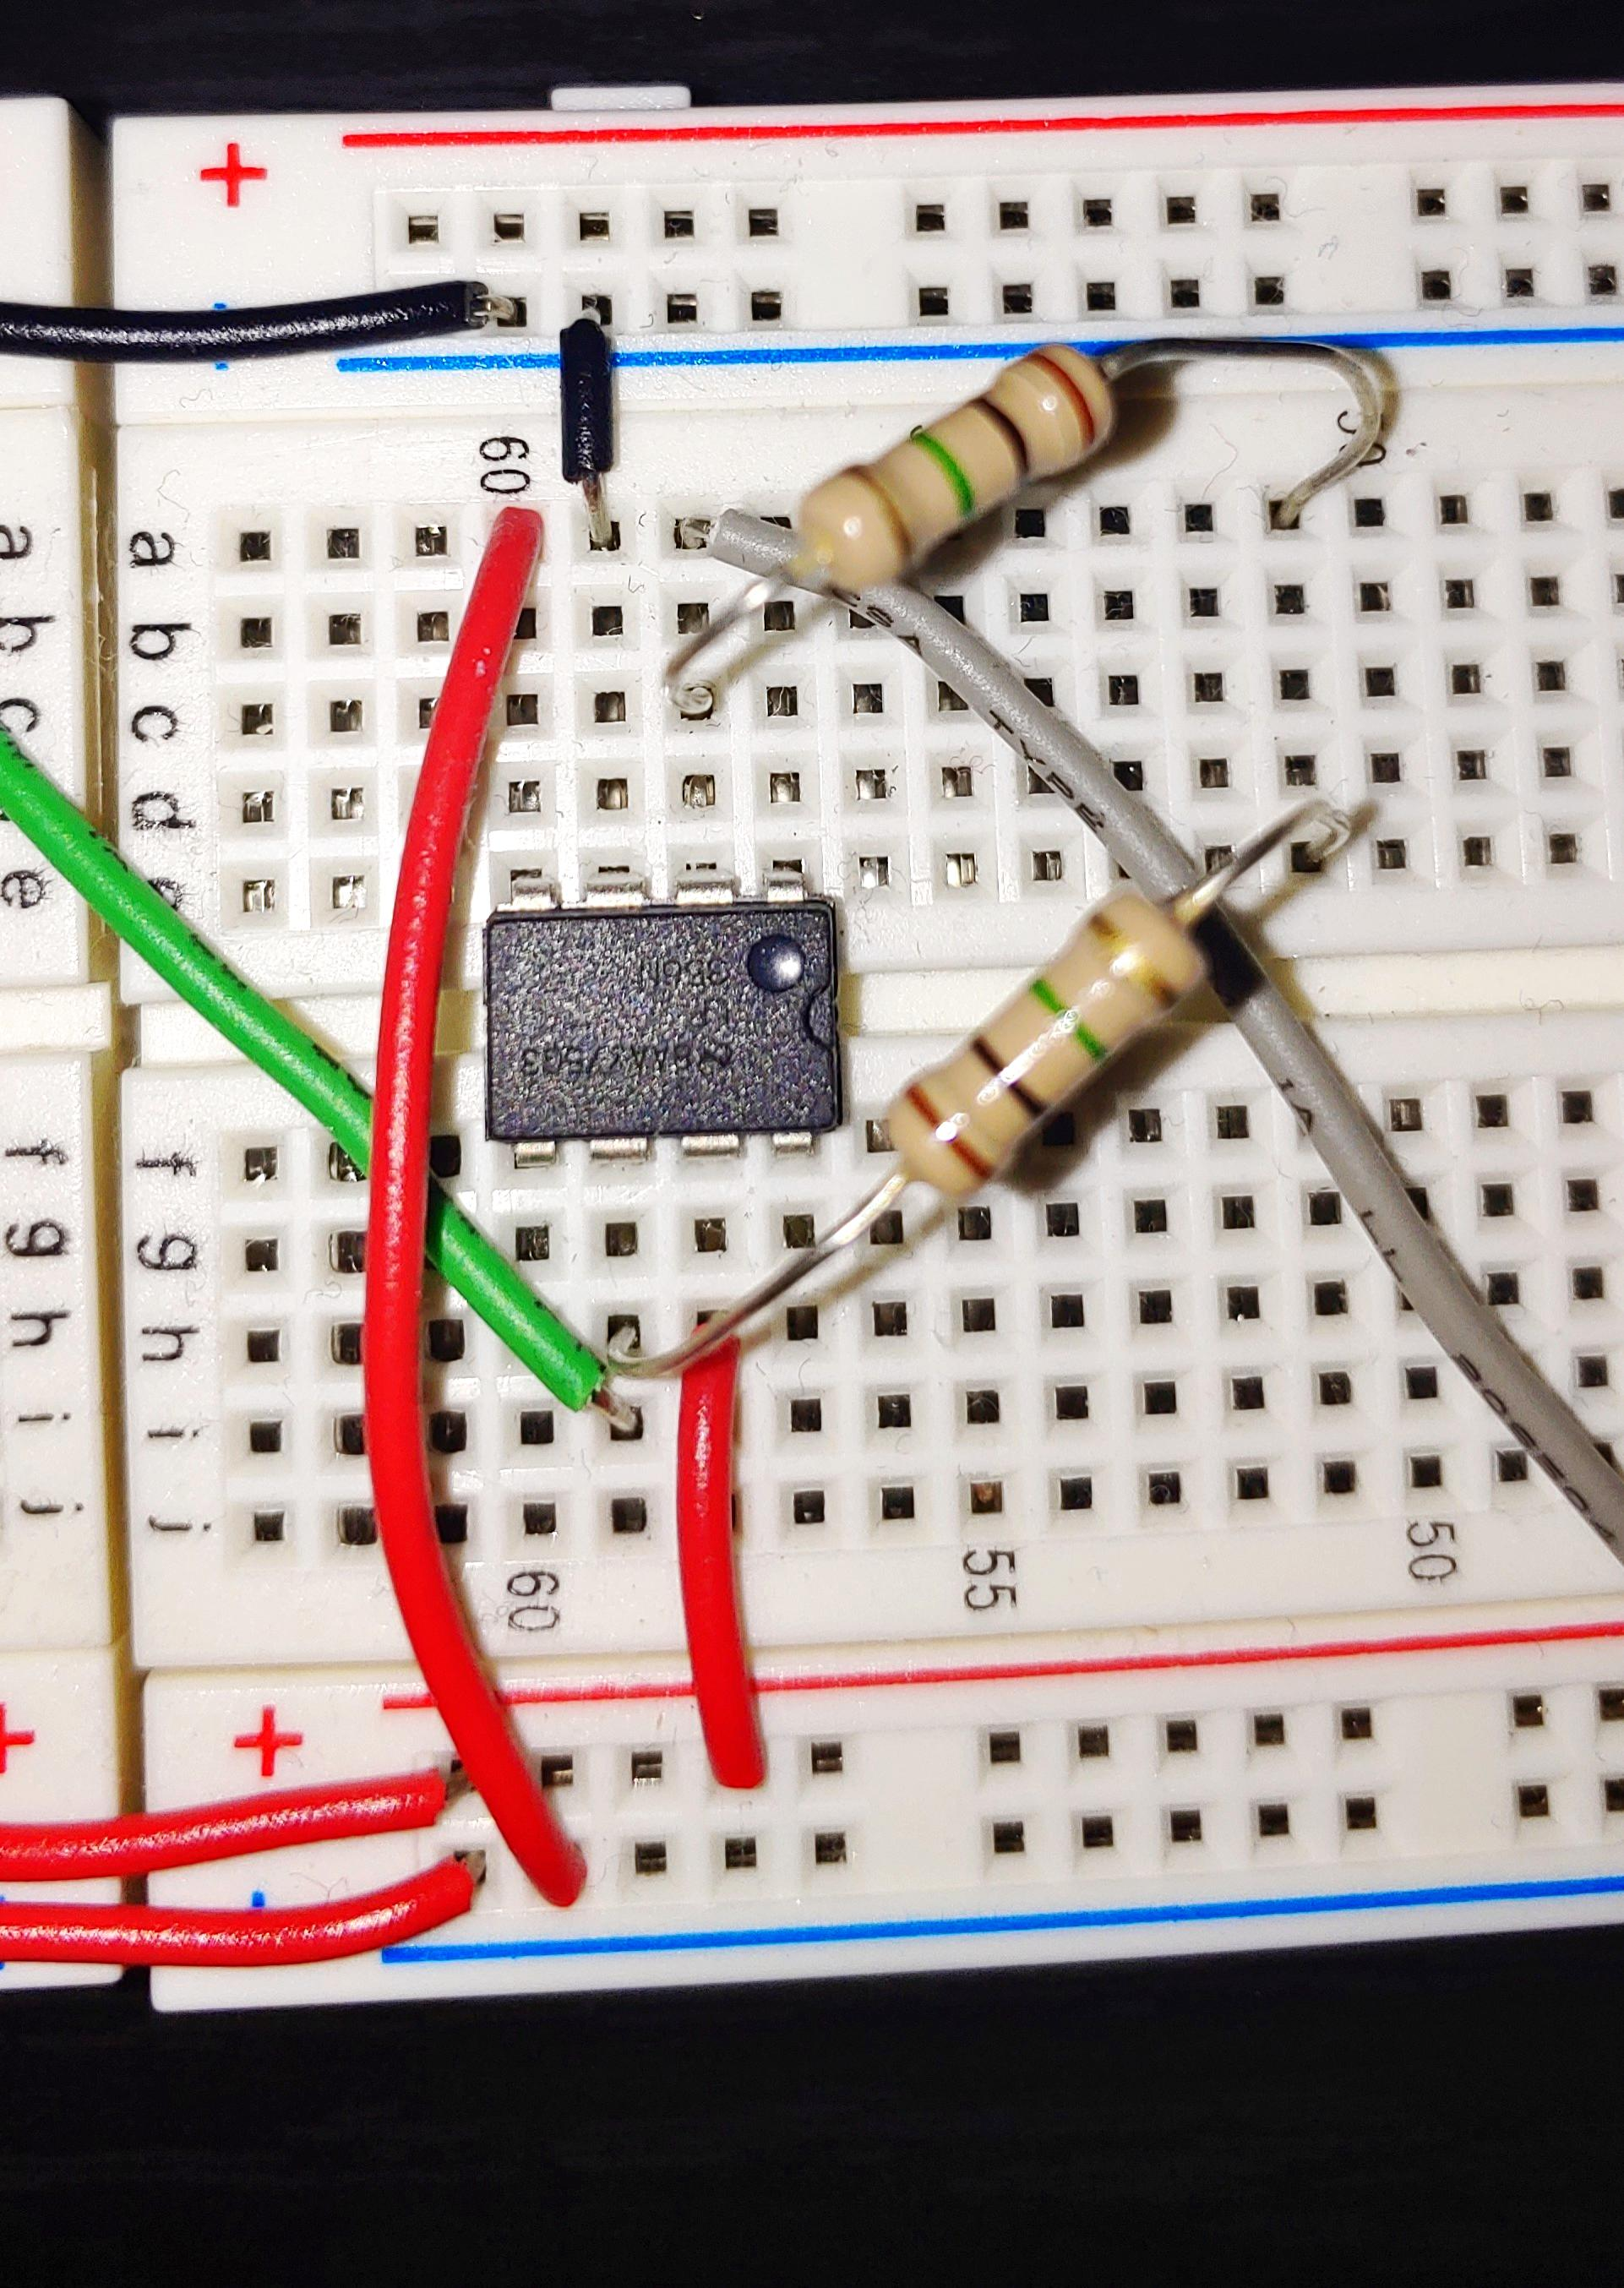
\includegraphics[width = .475\textwidth]{images/c_to_v_b.jpg}}
    \caption{The Built Current to Voltage Converter}
    \label{figure:BuiltCtoVCircuit}
\end{figure}
\newpage

Then the circuit when implemented with the output from the SpO2 sensor has an output seen in blue of (*Note the input is a current signal therefore the signal can not be seen by the AD2*):
\begin{figure}[h]
    \centering
    \boxed{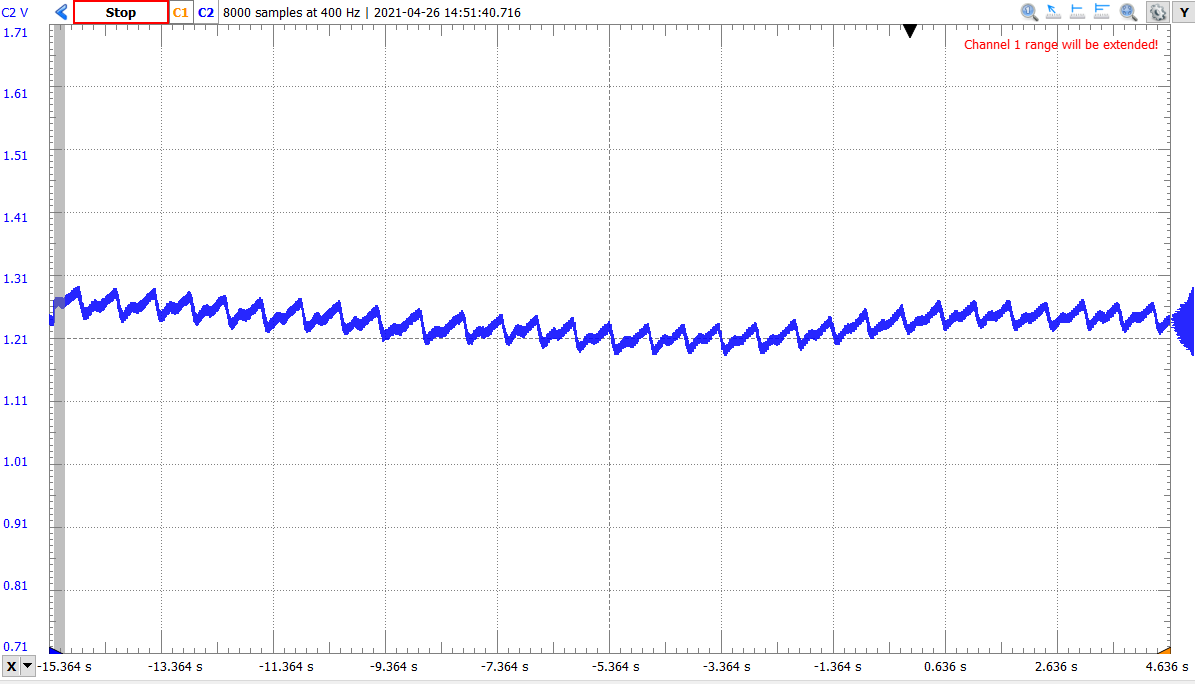
\includegraphics[width = \textwidth]{images/C_to_V_O.png}}
    \caption{Output from the Current to Voltage Converter in Blue with an Input from the SpO2 Sensor Output}
    \label{figure:CtoVBuiltOutputFromSpO2Sensor}
\end{figure}

This signal will then be taken to the next portion of the circuit with the filtering of the signal to reduce the noise seen clearly in \ref{figure:CtoVBuiltOutputFromSpO2Sensor}.
\newpage


\section{Filtering}
It was finally decided to use a two stage Bessel filter which will be sure to get rid of any noise and 60Hz hum very quickly. There was a $A_v$ gain of 0, and a cutoff frequency of $f_b = 3Hz$ which would get rid of unwanted parts of the AC signal.

The Filter Design Tool by Analog was use for this occasion:

\url{https://tools.analog.com/en/filterwizard/}
\begin{align}
    f_b &= 3Hz \\
    &= \frac{1}{2\pi RC}\\
    Let\text{ }&C = 1\mu F\\
    R &= \frac{1}{2\pi f_bC}\\
    &= \frac{1}{2\pi \cdot3Hz \cdot 1\mu F}\\
    &= 53051.65\Omega
\end{align}
Using their tool the user could input the desired passband and stopband values and component values $R = 56k\Omega$ and $C = 1\mu F$ were obtained. Now, building the circuit in LTSpice after rounding component values to those available in the kit, and test it there.
\begin{figure}[h]
    \centering
    \boxed{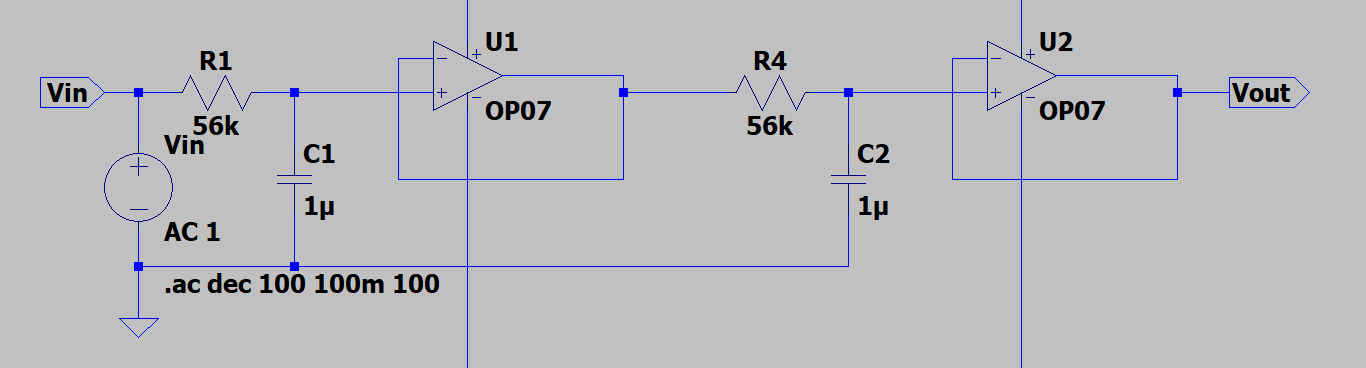
\includegraphics[width = .9\textwidth]{images/ltfilter_final.png}}
    \caption{LTSpice Schematic of the Complete Filters}
    \label{figure:LTSpiceFilters}
\end{figure}

Now, with a LTSpice diagram the circuit can be tested using a simple frequency sweep to get the bode plot for the circuit.
\begin{figure}[h]
    \centering
    \boxed{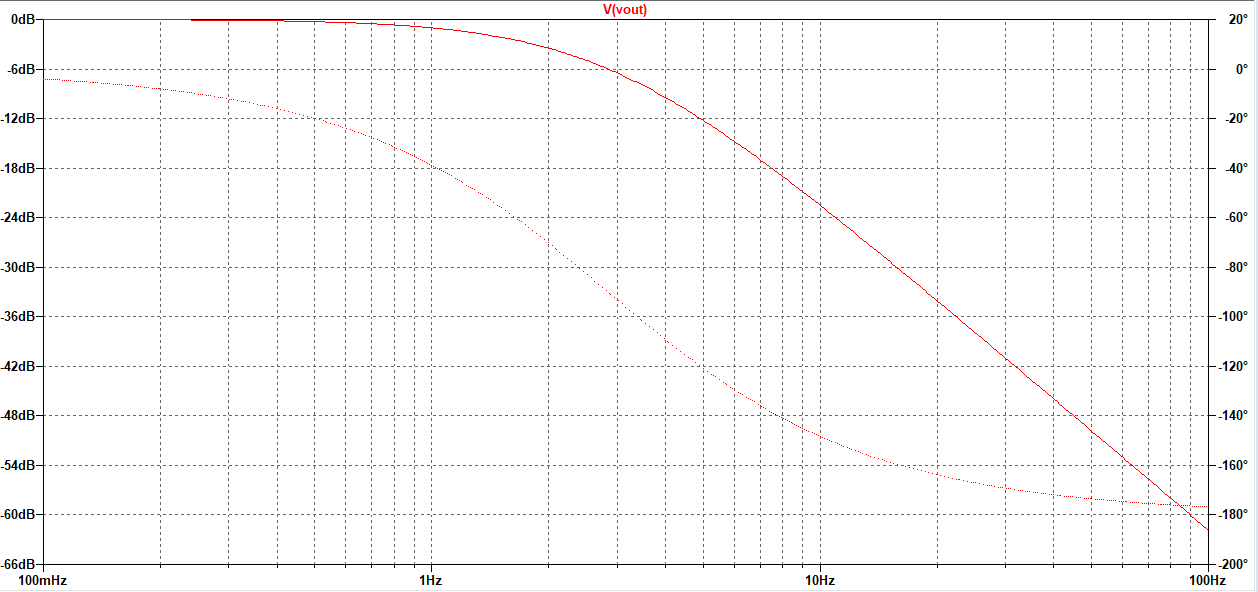
\includegraphics[width = .95\textwidth]{images/ltbodewhite.png}}
    \caption{Bode Plot of LTSpice Schematic of Filters}
    \label{figure:LTSpiceFilterBode}
\end{figure}
\newpage
Next, the circuit can be built in real life with the final result being:
\begin{figure}[h]
    \centering
    \boxed{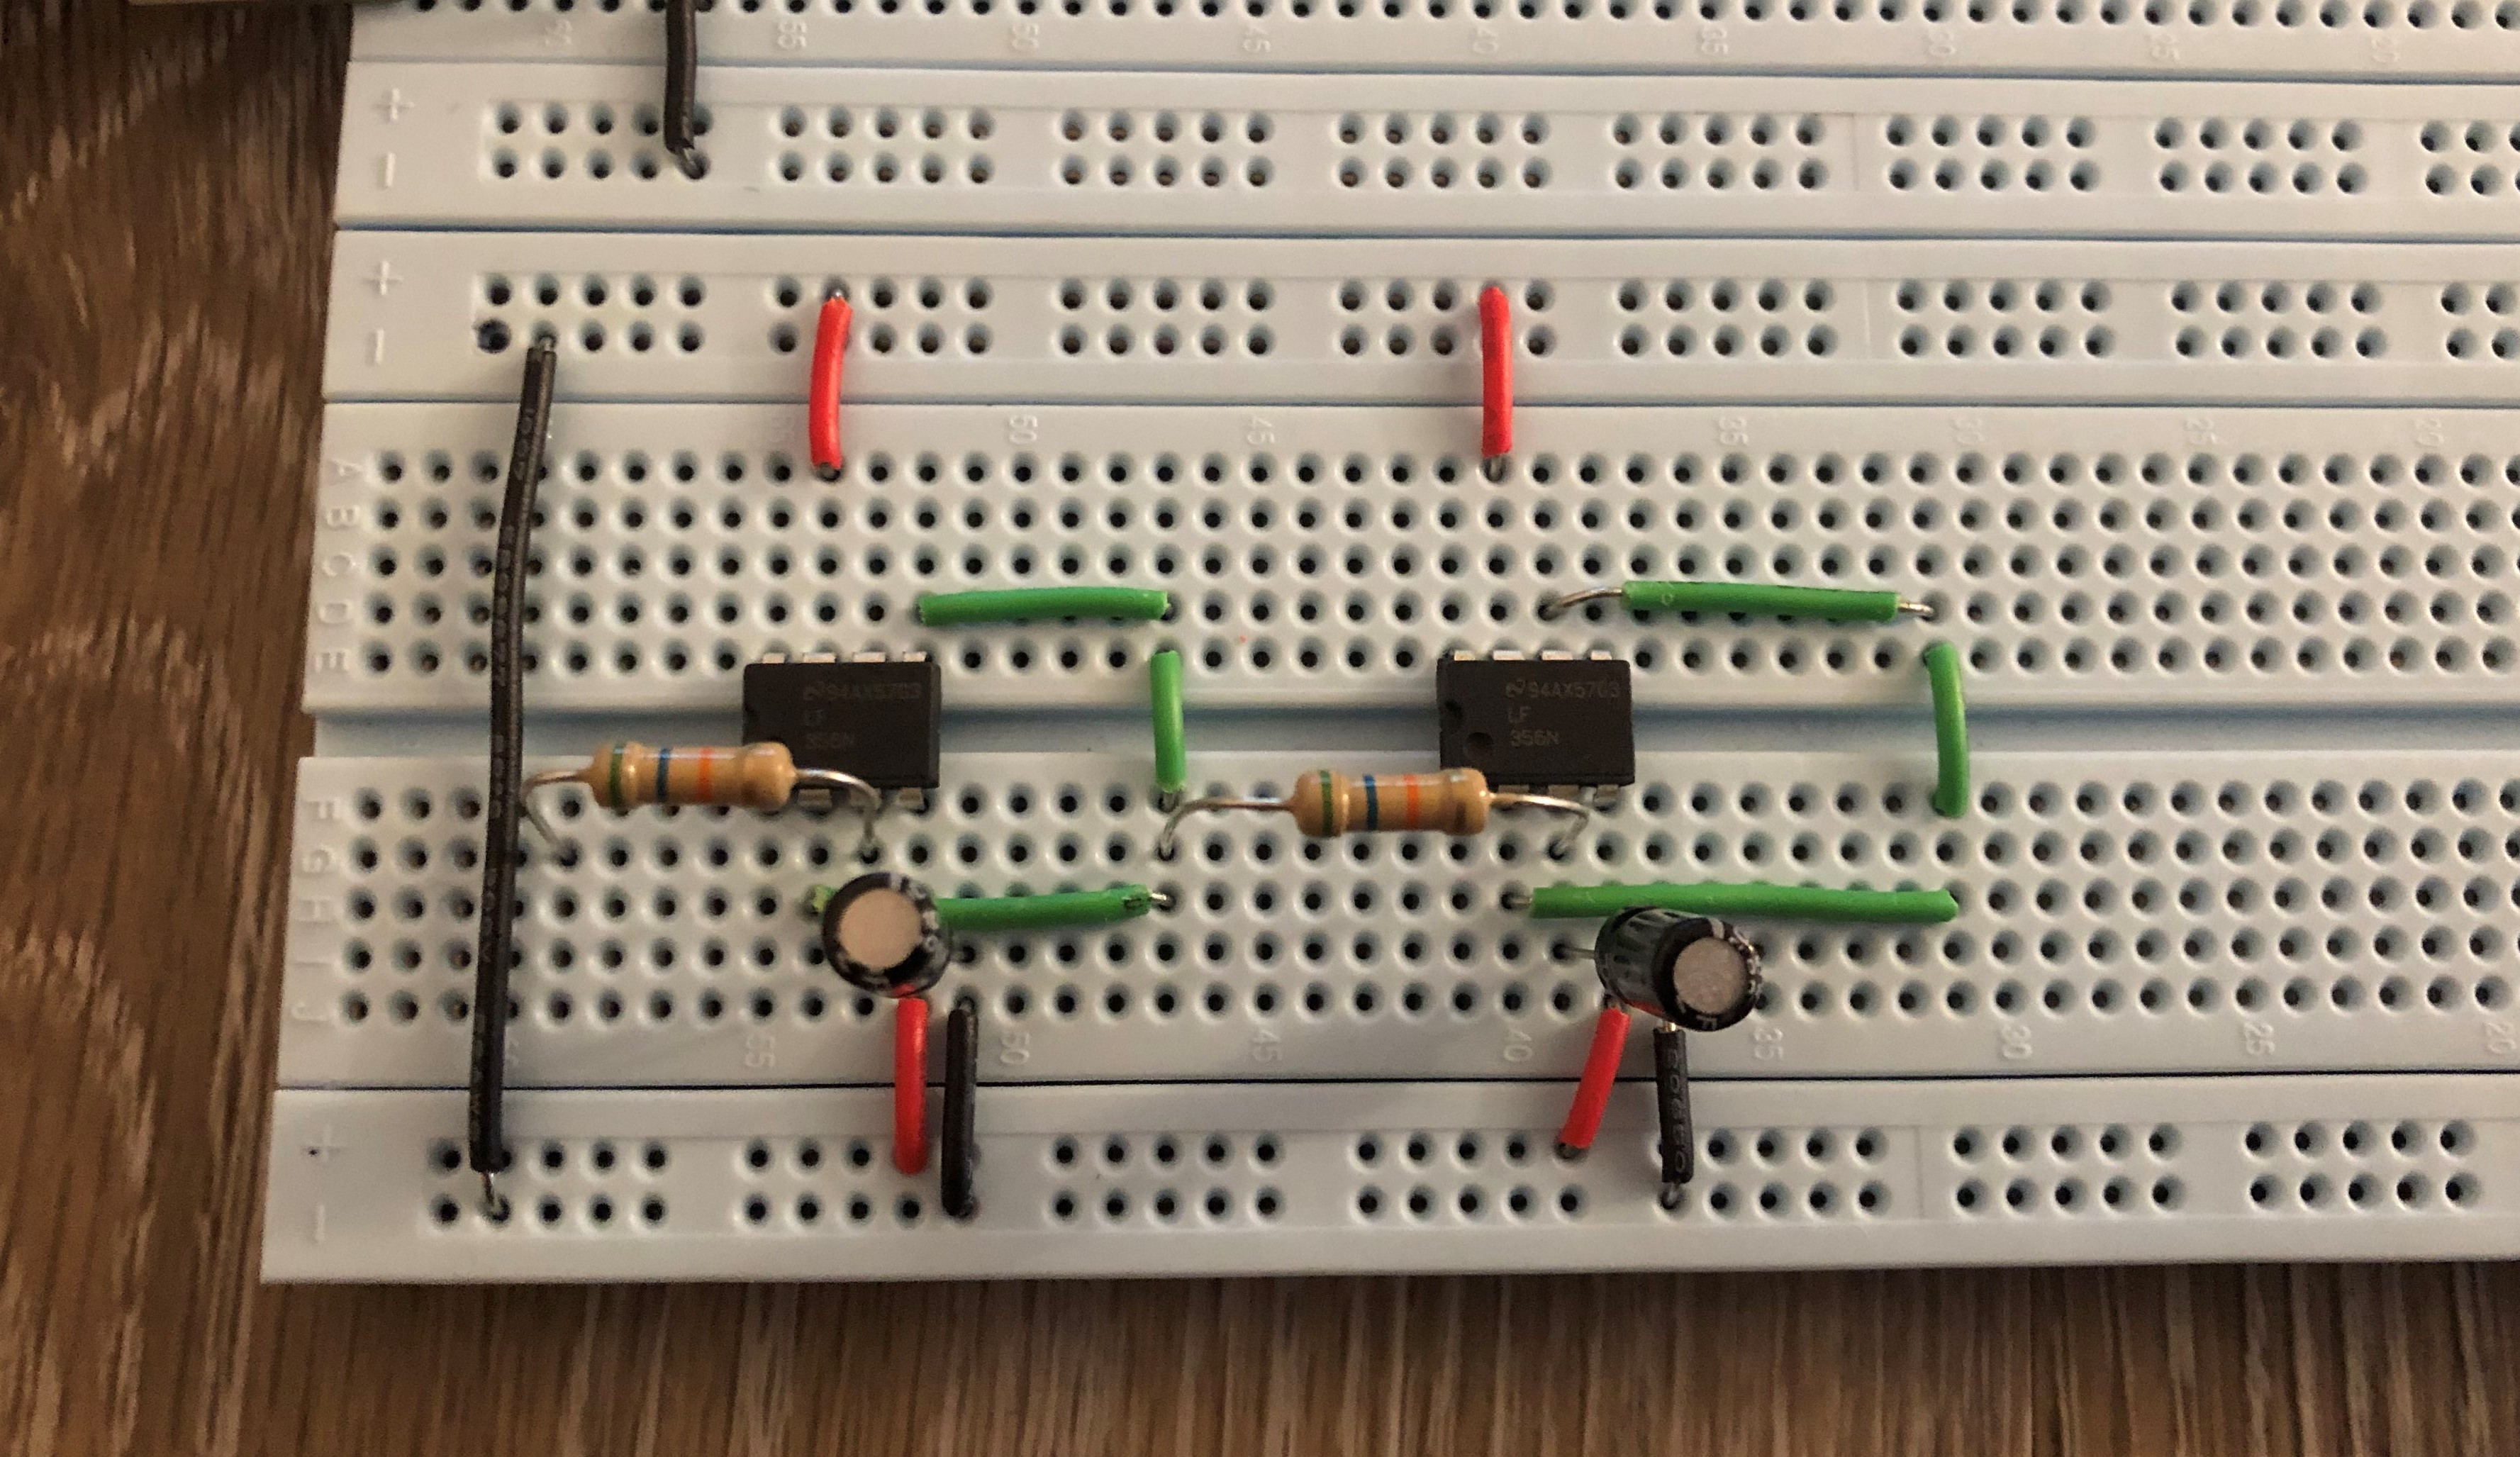
\includegraphics[width = .75\textwidth, height = .4\textwidth]{images/double_filter.jpg}}
    \caption{The Built Filter Circuit}
    \label{figure:BuiltFilter}
\end{figure}

Now with the circuit built, using the AD2 network analyser and a couple leads to obtain the bode plot of the circuit:
\begin{figure}[h]
    \centering
    \boxed{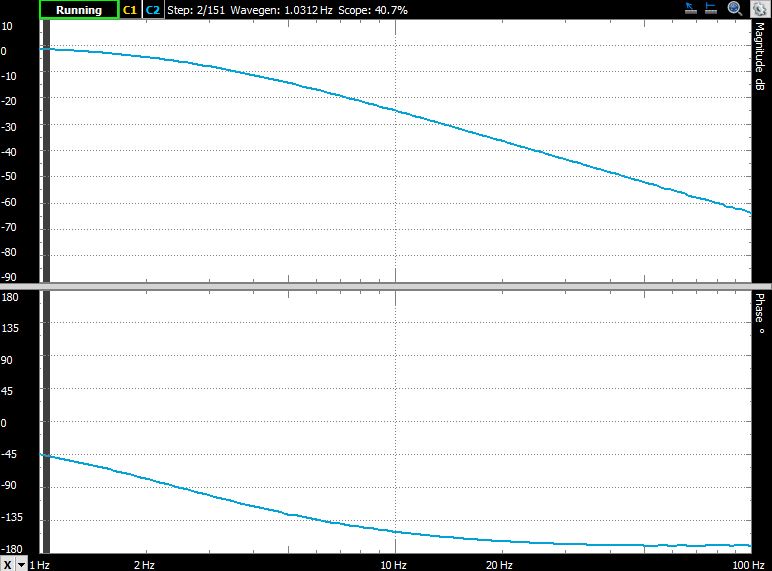
\includegraphics[width = .8\textwidth]{images/bodewhite.png}}
    \caption{The Built Filter Bode Plot Using AD2}
    \label{figure:BuildFilterBodePlot}
\end{figure}
\newpage
A break frequency, $f_b$, of 10Hz was chosen due to issues of the 1Hz signal being attenuated at 3Hz. Thus resulting in the final output signals with the unfiltered being on the left and filtered on the right.
\begin{figure}[h]
    \centering
    \boxed{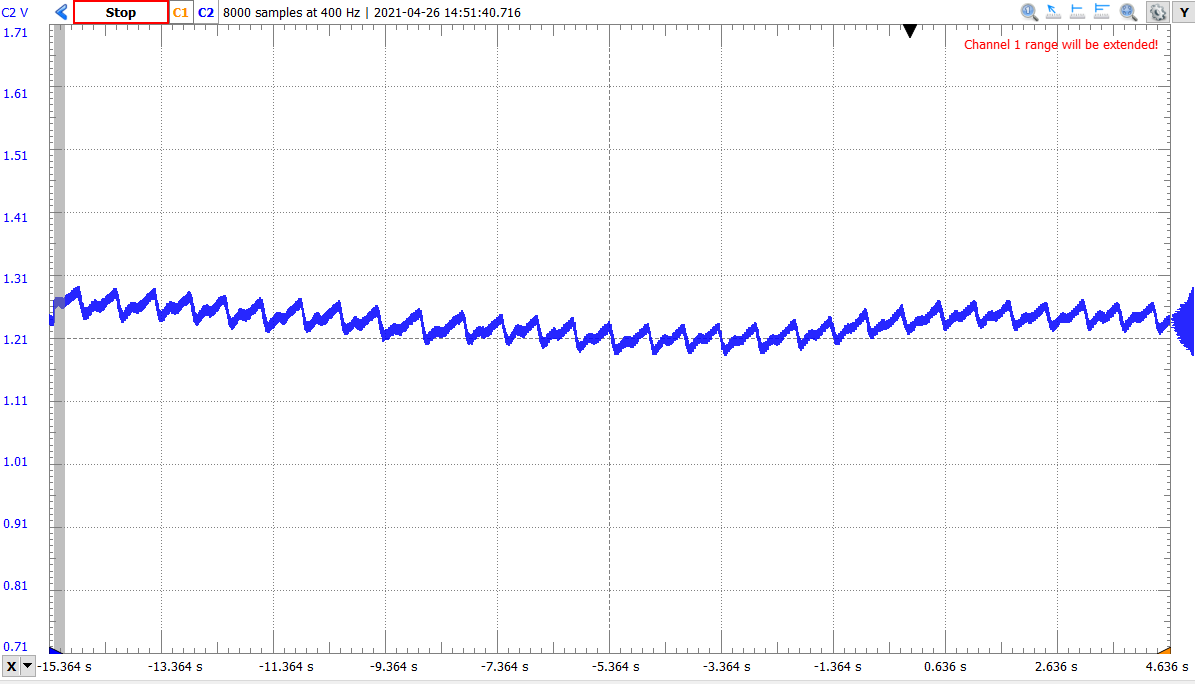
\includegraphics[width = .8\textwidth]{images/C_to_V_O.png}}
    \boxed{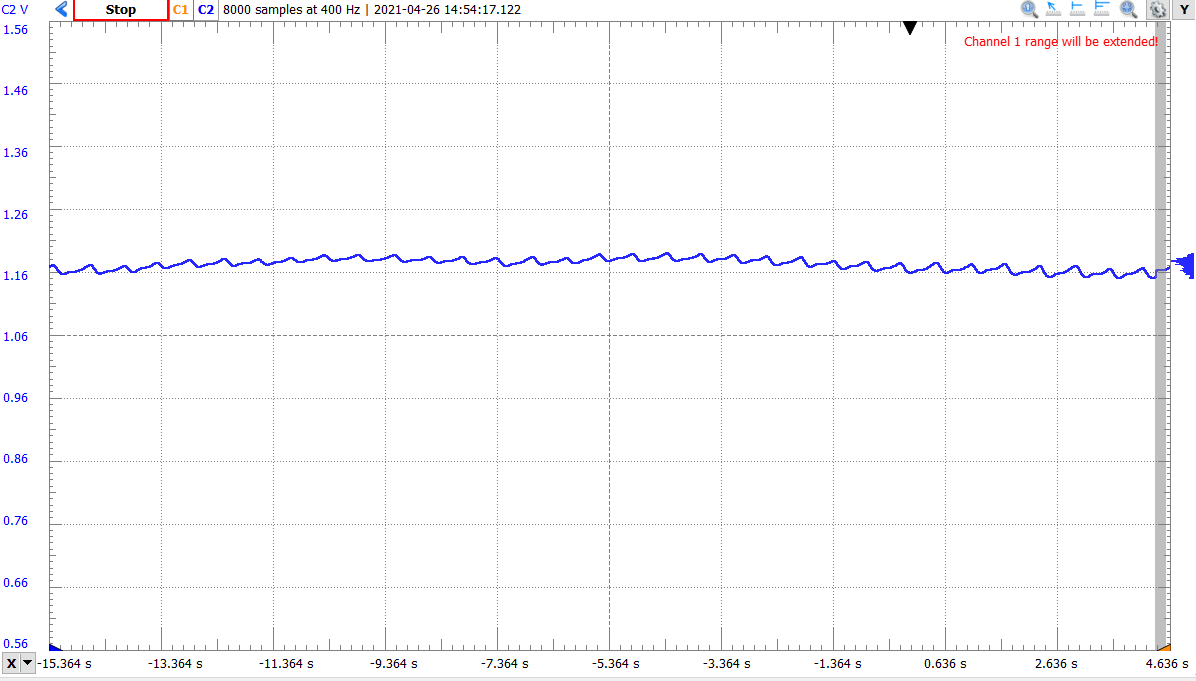
\includegraphics[width = .8\textwidth]{images/Filter_O.png}}
    \caption{The Unfiltered PPG Signal on Top and Filtered PPG Signal on Bottom}
    \label{figure:FilteredandUnfilteredSignal}
\end{figure}

Now, with a filtered PPG signal it is much easier to read and will give more information than before, for example with the differentiating circuit there will not be issues as there are no longer high frequency components that would constantly be hitting zero.
\newpage


\section{Post-Filtering Amplification}
After filtering the signal it was realized that the signal was still too small thus additional amplification was needed. Thus, with inspiration from [5] it was decided that a simple op-amp amplifier was used to be used to amplify the signal after the filtering of the signal. Using the information given in [5] the circuit below was created:
\begin{figure}[h]
    \centering
    \boxed{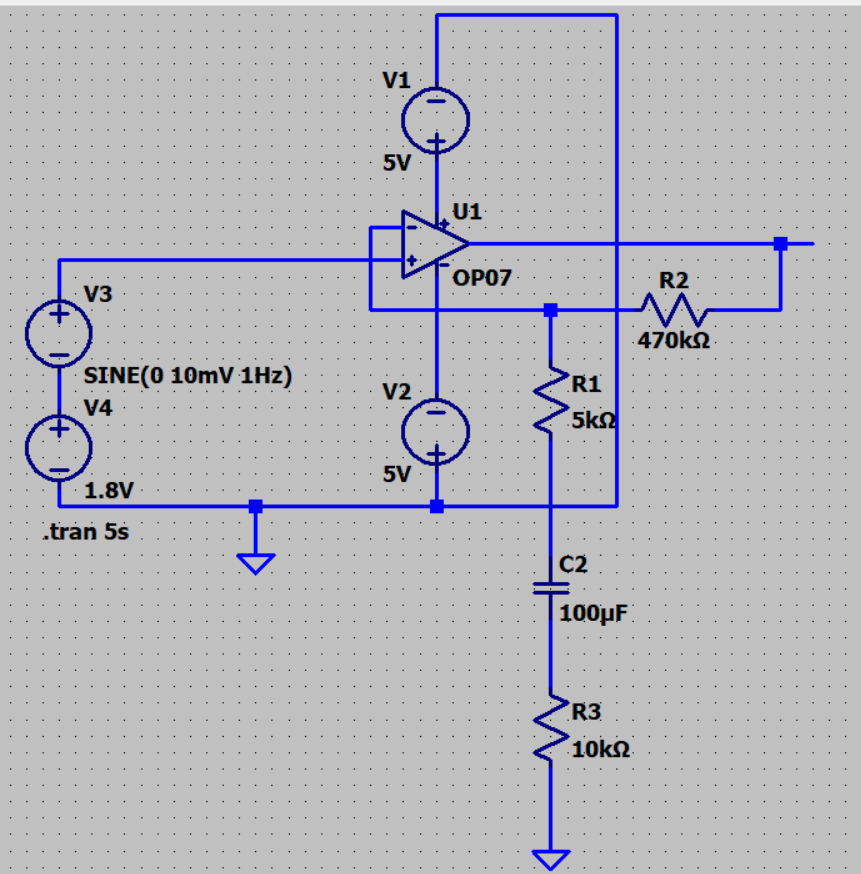
\includegraphics[width=\textwidth]{images/Op-Amp Amplifer.png}}
    \caption{LTSpice Schematic of Post-Filtering Amplifier Using Op-Amp Inspired by [5] in Appendix}
    \label{figure:PostFilterAmpLTSpice}
\end{figure}
\newpage

The amplifier circuit seen above takes the idea of a non-inverting op-amp amplifier and adds some changes to amplify the AC signal but not the DC signal. The amplification equation is still ruled by the basic equation of A\textsubscript{O} = (1 + R\textsubscript{F}/R\textsubscript{1}) but the equation is now different between AC and DC signals. 
In DC conditions, it can be see the coupling capacitor will be a open circuit thus causing the equation to be:
\begin{align}
A_{O} &= (1 +\frac{R_{1}+R_{2}+R_{3}}{R_{1} + R_{3}}) \\
A_{O} &= (1 +\frac{485k\Omega}{\infty\Omega}) \\
A_{O} &= (1 + 0) \\
A_{O} &= 1
\end{align}
Therefore the gain for DC conditions in this circuit is unity(aka. 1).
In AC conditions, it can be see the coupling capacitor will be a short circuit thus causing the equation to be:
\begin{align}
A_{O} &= (1 +\frac{R_{1}+R_{2}+R_{3}}{R_{1} + R_{3}}) \\
A_{O} &= (1 +\frac{485k\Omega}{10k\Omega + 5k\Omega}) \\
A_{O} &= (1 + 32.333) \\
A_{O} &= 33.333
\end{align}
Therefore the gain for AC conditions in this circuit is around 33.333.
It is know from testing the output from the filter is an AC signal with an amplitude of around 10mV riding on a DC voltage of around 1.8V.
This is simulated in the circuit above with the result from gain equations solved above being for DC:
\begin{align}
V_{O} &= A_{O} * V{in} \\
V_{O} &= 1 * 1.8V \\
V_{O} &= 1.8V
\end{align}
For AC:
\begin{align}
V_{O} &= A_{O} * V{in} \\
V_{O} &= 33.333 * 10mV \\
V_{O} &= 333.333mV
\end{align}
These are possible because of how the circuit is built with the circuit under DC conditions causing C2 to be open due to how capacitors work in DC conditions. This causes path to be blocked with a near infinite resistance therefore there is no gain under DC conditions. This is different under AC conditions with the capacitor now seen as a short circuit thus allowing for the amplification of the AC signal due to R1, R2, and R3 with the equations above. This is done to allow for the amplification of only the small AC signal without causing an amplification of the DC signal which at around 3.5V "overloads" the AC signal causing the signal to become DC. 
\newpage
This leads to final result LTSpice simulation for the circuit above of:
\begin{figure}[h]
    \centering
    \boxed{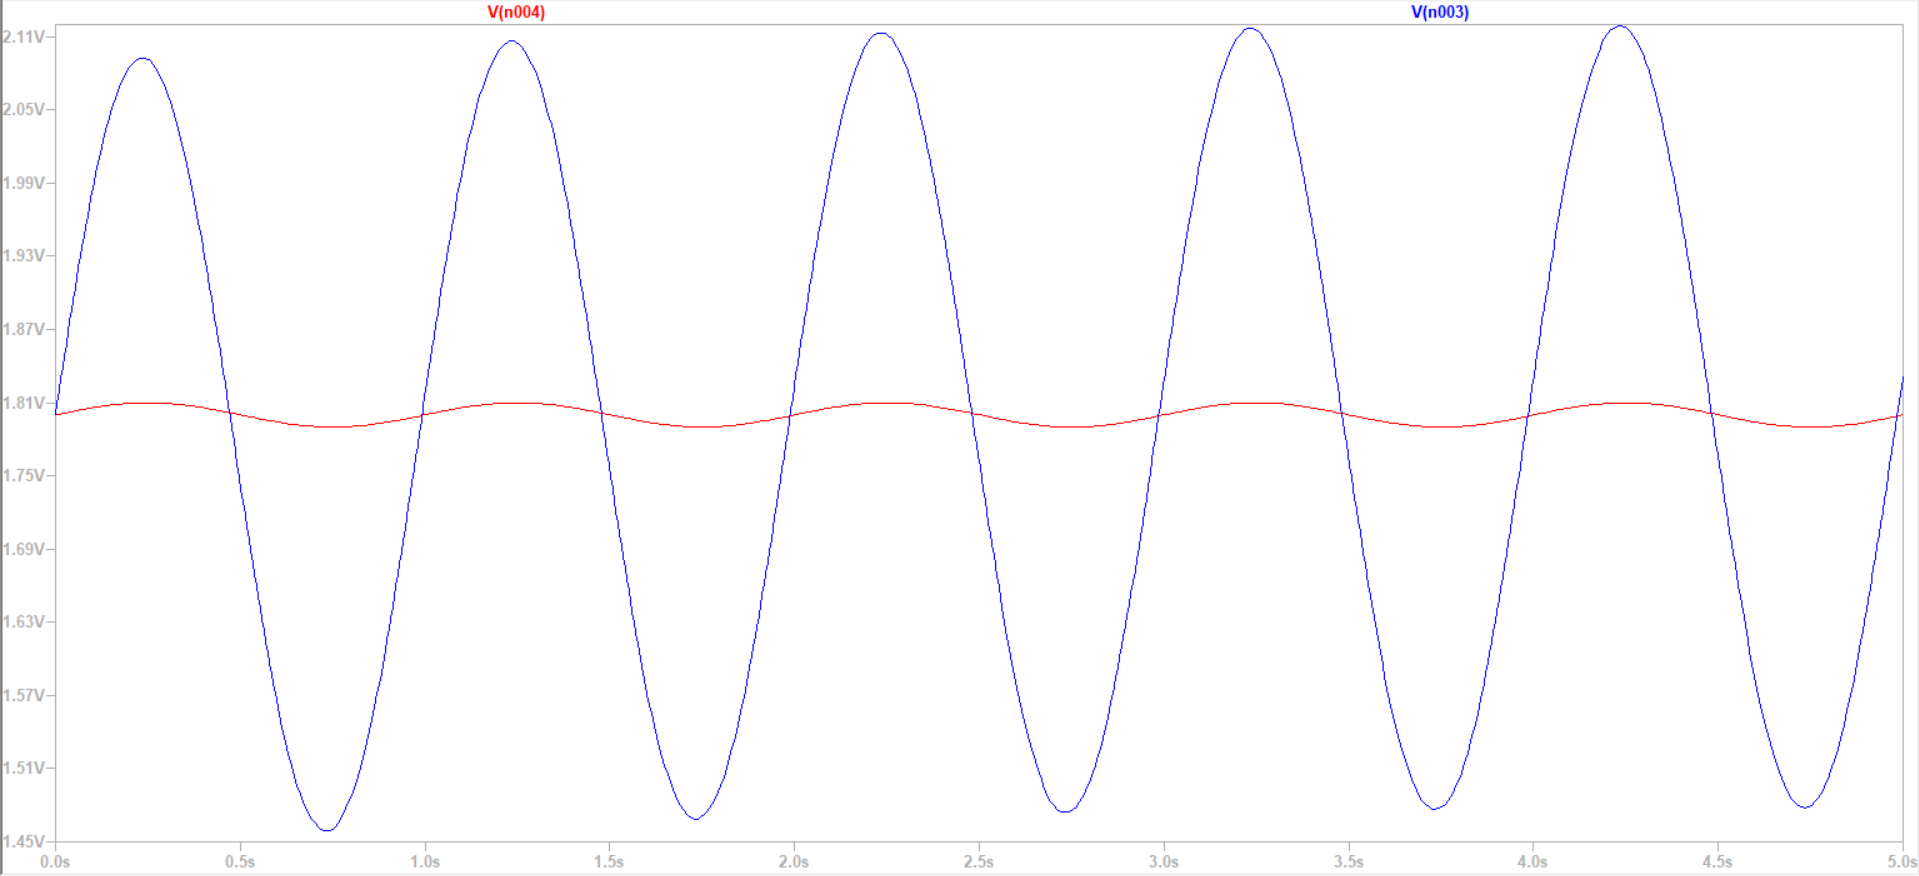
\includegraphics[width=\textwidth, height = .5\textwidth]{images/Op-Amp Amplifer_O.png}}
    \caption{LTSpice Simulation of Post-Filtering Amp. from \ref{figure:PostFilterAmpLTSpice} with Input Seen in Red and Output Seen in Blue}
    \label{figure:PostFilterAmpLTSpice_O}
\end{figure}

The circuit when implemented with the overall circuit with an addition of a diode to not go above the -0.6V limit of the Arduino resulted in:
\begin{figure}[h]
    \centering
    \boxed{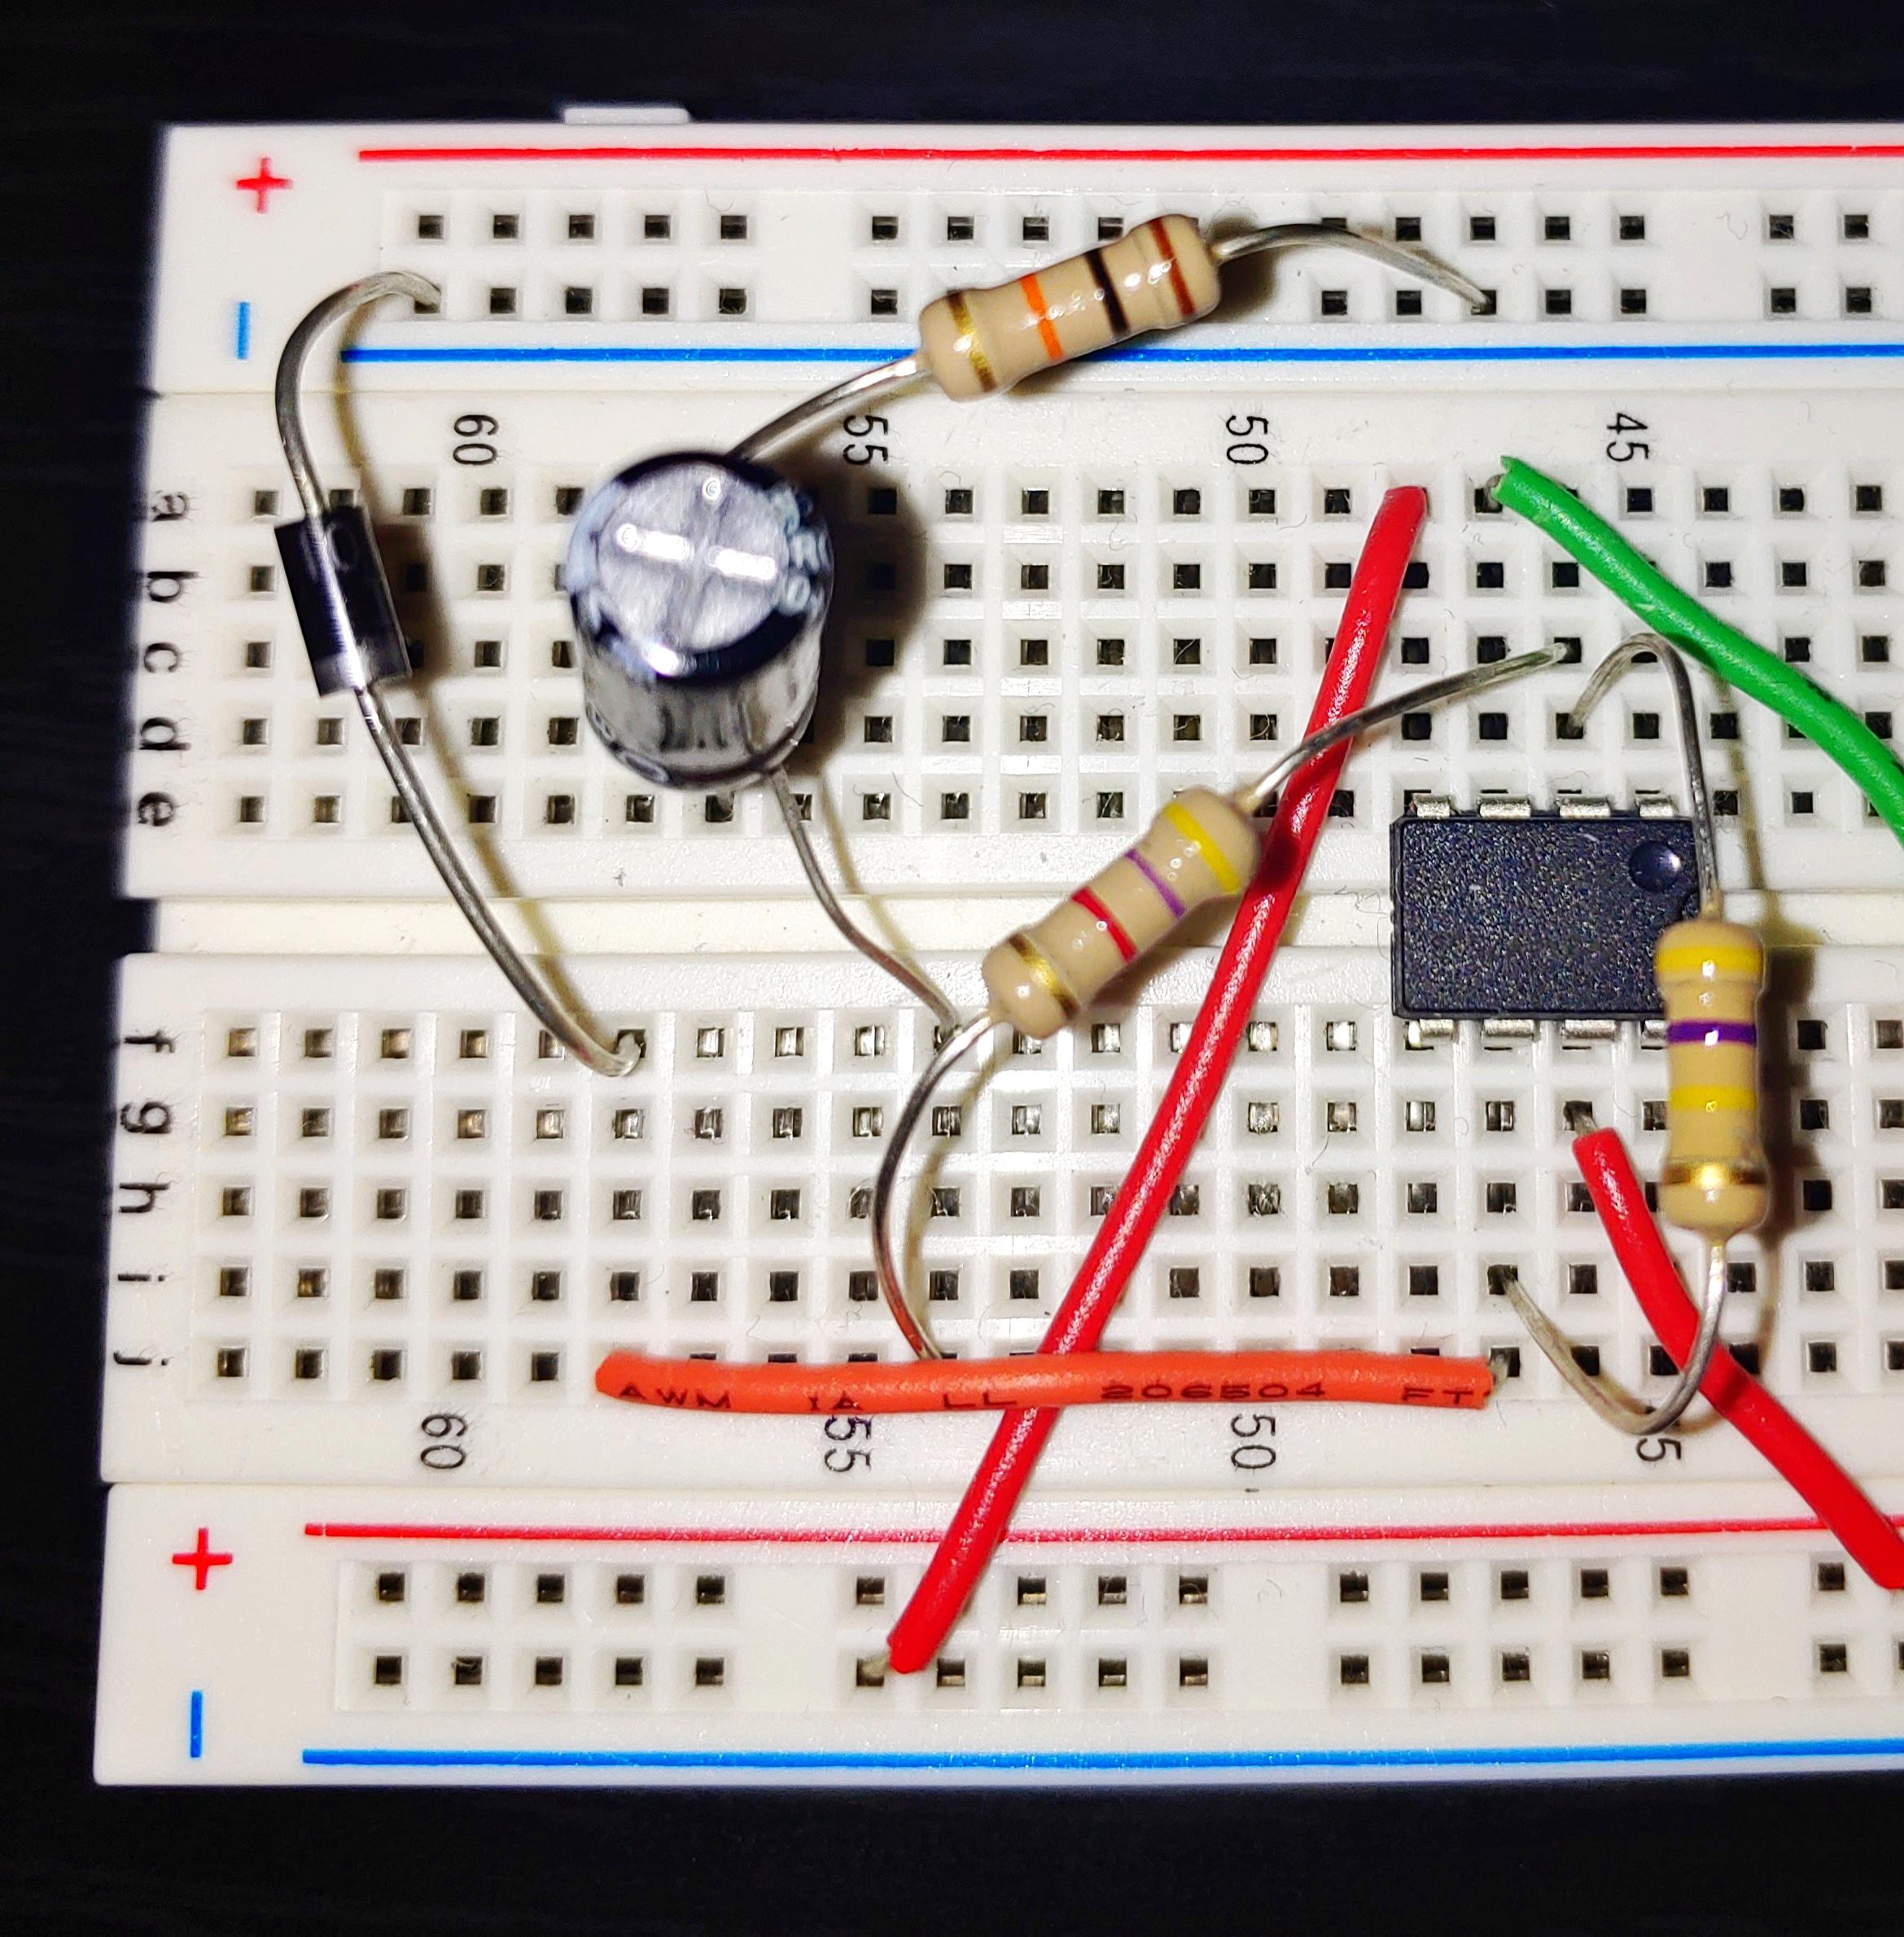
\includegraphics[width = .75\textwidth, height = .45\textwidth]{images/Post_F_Amp_b.jpg}}
    \caption{The Built Post-Filtering Amplifier Connected to Filter Output}
    \label{figure:Post-FilterAmpBuilt}
\end{figure}

\newpage
The final output of the overall circuit/system is seen with a addition of a diode to ground as given advice to make sure that the signal does not go above the -0.6V limit on the Arduino pins causing the pins to get "popped". The final output of the overall circuit after that is seen to be:

\begin{figure}[h]
    \centering
    \boxed{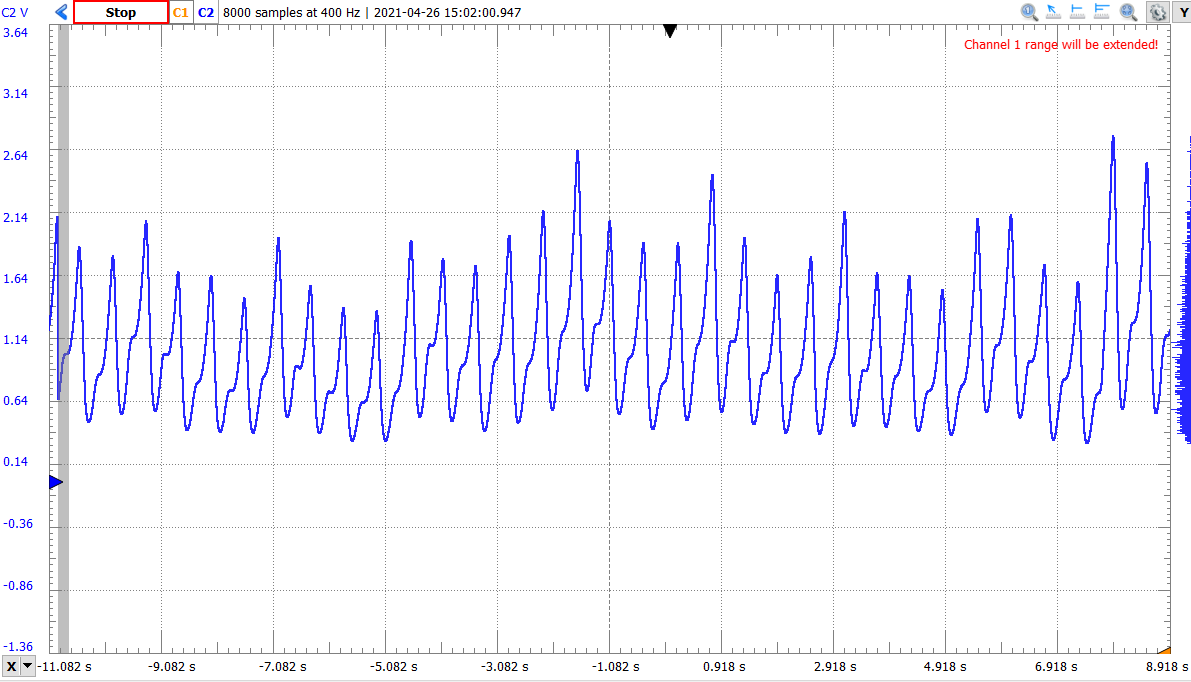
\includegraphics[width = \textwidth, height = .5\textwidth]{images/Post-Filter_Amp_D_O.png}}
    \caption{The Output in Blue of the Built Post-Filtering Amplifier for Overall Circuit with Included Diode}
    \label{figure:Post-FilterAmpBuilt_O}
\end{figure}

The figure above Figure \ref{figure:Post-FilterAmpBuilt_O} is seen to be the final signal after processing and will now be used to calculated heart rate and SpO2 values in the upcoming sections.

\newpage
\section{Calculating Heart Rate}
Now, to calculate the heart rate an algorithm will be used to detect peaks. It involved storing the data inputs, and based on their magnitudes relative to each other the code decides if there is a peak or not, and by storing the time that the last couple beats occurred and plugging it into the a formula that calculates the amount of beats per minute based on those beat timings.

The way it detects a peak is by checking if the function has been constantly increasing for a certain amount of time, by fine tuning this amount we can successfully identify every peak that come across

Then by recording the time at which each beat occurs and storing the past times, we can calculate a rolling average of the different beat times such that we have an average period, using a simple formula:
\begin{equation}
    \text{BPM (beats per minute)} =  \frac{60s}{T}
\end{equation}
The BPM of the signal can now be found as shown by the sample code below.
\begin{lstlisting}[language=Arduino, caption= HR Calculation Code]
void calcHR(){
  oldT[heartrateptr] = millis() - last_beat;  //subtracts current time from time since last beat to get period
  last_beat = millis();                       //sets current time to last beat in preperation for next cycle
  
  //calculates average period and R value using last couple values calculated
  int avPeriod = 0;
  for(int i =1; i<SAMPLES_STORED; i++) {
        avPeriod += oldT[i];
        avR += oldR[i];
  }
  
  //updates pointer used to store data points in array
  heartrateptr++;
  heartrateptr %= SAMPLES_STORED;
  
  avR /= SAMPLES_STORED ;
  avPeriod /= SAMPLES_STORED;
  // 60000 (60 seconds in milliseconds) / (averagePeriod) and this give beat per minute 
  avBPM = 60000 / (avPeriod) ;
}
\end{lstlisting}
A benefit of having the code structured like this is that if the value of the heart rated was wanted to be more smooth all that would be need to do is change the sample size at the start of the file and it will store more beat timings to take the average of and therefore be more smooth since its averaging over a larger period of time.

The accuracy of this was tested by testing it against an Apple watch, and using the SpO2 sensor and comparing the readings and they came out to be quite close, in fact the apple watch was slightly worst as it updated less frequently and was often behind on its reading.
\newpage


\section{Calculating SpO2}
The first step in calculating SpO2 is to calculate the R ratio which relates the two wavelengths of light into one number which can be used to find SpO2. There are several acceptable methods to calculate the R ratio. The way decided to go about doing this was to find the maximum and minimum of a given period of the signal which was stored in an array and use those values for the calculation, the code snippet for this can be seen below.
\begin{lstlisting}[language=Arduino, caption= R Calculation Code]
void calcR(){
    //having these values at the min and max makes sure that the values read from the array will replace the initial ones since they must be larger or smaller than min or max
    maxInfared = 0; 
    maxRed = 0; 
    minInfared=MAX_ADC_VALUE; 
    minRed=MAX_ADC_VALUE;
    // Iterate through the array, if value is bigger than current max, it becomes new max opposite is true for minimum, by the time the loop is over we have max and min
    for(int i=0;i<SAMPLES_PER_PERIOD;i++) {
      if(IRarray[i]> maxInfared){
        maxInfared = IRarray[i];
      } 
      if(IRarray[i]>0 && IRarray[i]< minInfared ){
        minInfared = IRarray[i];
      }
      if(Rarray[i]> maxRed){
        maxRed = Rarray[i];
      }
      if(Rarray[i]>0 && Rarray[i]< minRed ){
        minRed = Rarray[i];
      }
      IRarray[i]=0;
      Rarray[i]=0;
    }
    R = ((maxRed-minRed)/minRed)/((maxInfared-minInfared)/minInfared);
}
\end{lstlisting}
Now, that the R value is stored. For, it to be able to find the SpO2 values, there needs to be a little bit of background on how to do that. The curve for the relation between the R ratio and the SpO2 value can be seen below.
\begin{figure}[h]
    \centering
    \boxed{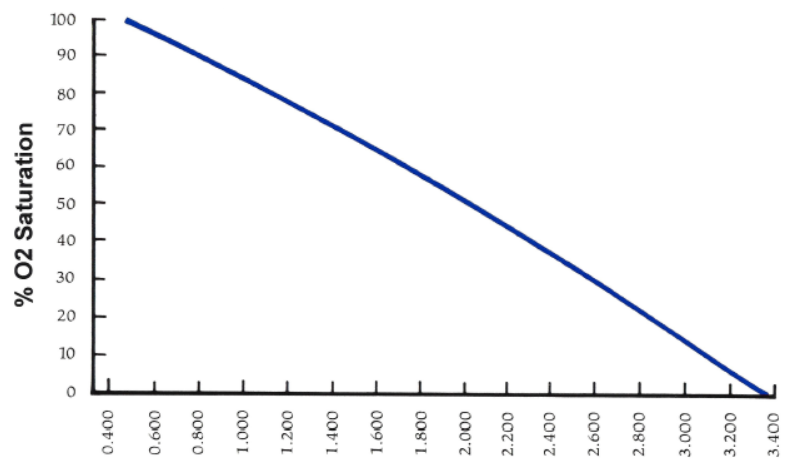
\includegraphics[width = .6\textwidth]{images/rvsspo2.png}}
    \caption{R Vs. SpO2 Values as a Linear Graph}
    \label{figure:SpO2LinearGraph}
\end{figure}
As can be seen it is not an easy graph to represent with code, so the next best solution is to use a linear approximation for this curve since it is very straight as is, when we do that we get the linear equation:
\begin{equation}
    \text{SpO2} = -19 * R + 114;
\end{equation}
\newpage
\section{Information Display}
One of the objectives of this project is to display the sensor output after it has been processed on to the LCD screen, the code for this and an example picture of what it looks like is below:
\begin{figure}[h]
    \centering
    \boxed{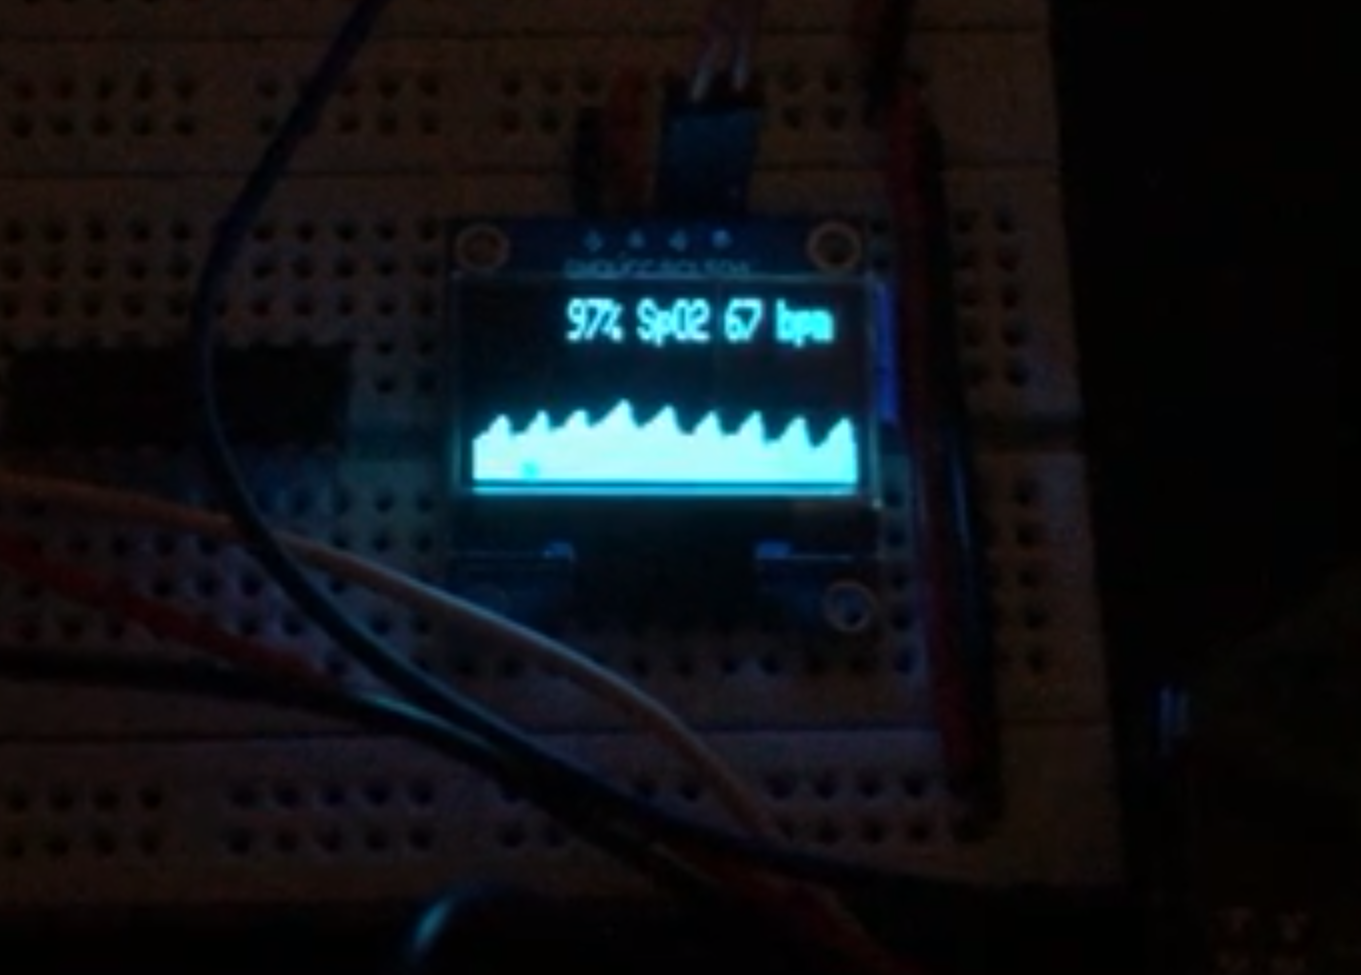
\includegraphics[width = .7\textwidth, height = .4\textwidth]{images/displayexample.png}}
    \caption{Display with Heart Rate and SpO2 Values along with Input Signal}
    \label{}
\end{figure}
\begin{lstlisting}[language=Arduino, caption= Display Code]
//resets print pointer if it has reached the edge of the display
if(printptr >= display.width()){
 printptr = 0;
}
// reads value from analog pin 
int analogVal = analogRead(sensorPin);

//puts value into array 
circularBuffer[printptr++] = analogVal;

//for loops to draw the graph itself
int xPos = 0; 
for (int i = printptr; i < display.width(); i++){
 int analogVal = circularBuffer[i];
 drawLine(xPos, analogVal);
 xPos++;
}
for(int i = 0; i < printptr; i++){
 int analogVal = circularBuffer[i];
 drawLine(xPos, analogVal);
 xPos++;;
} 

//helper function to draw graphs
void drawLine(int xPos, int analogVal){
  int lineHeight = map(analogVal, 0, MAX_ADC_VALUE, 0, graphHeight);
  int yPos = display.height() - lineHeight;
  display.drawFastVLine(xPos, yPos, lineHeight, SSD1306_WHITE);
}
\end{lstlisting}
This graph gives a good indication to the user if they are seating their finger properly on the sensor or not, and can not only see that heart rate in bpm but see that actual graph that the number is derived from.
\newpage


\section{Appendix}
\subsection{Complete Code}
Here I will provide the full code, which must be attached and does not contribute to the 30 page limit given.
\begin{lstlisting}[language=Arduino, caption= Complete Appendix Code]
/**
  ECE2804 SpO2 Sensor Code
  Name: project_code
  Purpose: calculate heart rate and SpO2 
            given cleaned signals from sensor

  @author Kavin Thirukonda
  @version 2.4 4/27/21
*/

//standard includes needed for display
#include <Wire.h> 
#include <SPI.h>
#include <Adafruit_GFX.h>
#include <Adafruit_SSD1306.h> 

//creating display object using screen size parameters
#define SCREEN_WIDTH 128 // OLED display width
#define SCREEN_HEIGHT 32 // OLED display height
Adafruit_SSD1306 display(SCREEN_WIDTH, SCREEN_HEIGHT, &Wire, -1);

//declaring graph printing variables
int circularBuffer[SCREEN_WIDTH]; 
int printptr = 0; 
int graphHeight = SCREEN_HEIGHT - 10;

//creating defines to use during programming to make code easier to read
#define SAMPLES_PER_PERIOD 60 
#define SAMPLES_STORED 10     
#define SMOOTHING 4           
#define BEAT_INDICATOR 12      
#define MEASURING_PERIOD 5
#define MAX_ADC_VALUE 1023

//preinitializing functions
void readRED();
void readIRED();
void calcR();
void calcHR();

//setting variables for pin locations
int sensorPin = A0; 
int REDLedPin = 3;
int IRLedPin = 4;
 
//variables needed for the bulk of calculations
float infaredIn[SMOOTHING], sumIR,lastIR, scanner, start;
float redIn[SMOOTHING], sumRED,lastRED;
int period, samples;
int samplesCounter = 0;
float infaredInSPO2[SAMPLES_PER_PERIOD],redInSPO2[SAMPLES_PER_PERIOD];
float maxInfared= 0;
float minInfared= 0;
float maxRed= 0;
float minRed= 0;
double R=0;
float oldR[SAMPLES_STORED];
int oldT[SAMPLES_STORED];
int spo2ptr = 0;
int heartrateptr = 0;
int readptr;
float avR = 0;
int avBPM=0;
int bpmprint;
int spo2print=0;
float beforeIR;
bool rising;
int riseDuration;
int n;
long int last_beat;

/**
  Setup function used to initialize certain variables to zero
  and set some settings.

  @param  none
  @return none
*/
void setup() {

   //Setting Baudrate of device
   Serial.begin(9600);

   //Ensuring buffer for  device is clear
   Serial.flush();

   //check if display is properly connected, if not stop program
   if (!display.begin(SSD1306_SWITCHCAPVCC, 0x3C)) { 
     Serial.println(F("SSD1306 allocation failed"));
     for (;;); // Don't proceed, loop forever
   }

   //initialize display by clearing startup
   //setting font and text color 
   //as well as initial drawing position
   display.clearDisplay();
   display.setTextSize(1);
   display.setTextColor(WHITE, BLACK);
   display.setCursor(0, 0);
   display.display();
   delay(500);
   display.clearDisplay();

   //Setting various modes on pins using previously declared 
   //variables and Arduino functions
   pinMode(sensorPin,INPUT);
   pinMode(REDLedPin,OUTPUT);
   pinMode(IRLedPin,OUTPUT);

   //Sets initial state of both LEDs to off
   digitalWrite(REDLedPin,LOW);
   digitalWrite(IRLedPin,LOW);

   //Initializes arrays to zero using memset function
   memset(infaredInSPO2, 0, SAMPLES_PER_PERIOD);
   memset(redInSPO2, 0, SAMPLES_PER_PERIOD);
   memset(oldT, 0, SAMPLES_STORED);
   memset(oldR, 0, SAMPLES_STORED);
   memset(infaredIn, 0, SMOOTHING);
   memset(redIn, 0, SMOOTHING);
   period=0; 
   samples=0;
   sumIR = 0; 
   sumRED=0; 
   readptr = 0; 
}

/**
  main program loop, contains all overarching logic for
  when certain numbers are calculated and the display logic.

  @param  none
  @return none
*/
void loop (){  
    //calls function to read RED LED, for more indepth explaination check appropriate funtion
    readRED();

    //calls function to read IRED LED, for more indepth explaination check appropriate funtion
    readIRED();

    //stores output from both previously called functions into an array which can be
    //processed to calculte SpO2
    infaredInSPO2[spo2ptr]=lastIR;
    redInSPO2[spo2ptr]=lastRED;

    //increments circular pointer used to fill the array which manages spo2 caluclations,
    //since the only information we need from this is the maximum and minimum values
    //order does not matter and placing them anywhere in the array works fine for us.
    spo2ptr++;
    spo2ptr %= SAMPLES_PER_PERIOD;

    //Increments counter to check how many "samples" have been taken, my definition of a 
    //sample is everytime the two readRED() and readIRED() functions are all called there
    //is new sample, it is the checked if the sample count is above a  threshold which will
    //be explained later, if it is then a new R value is caluclated.
    samplesCounter++;
    if(samplesCounter>=samples){
      //calls function to calculate R, for more indepth explaination check appropriate funtion
      calcR();  
    }

    //reset variables for average R value and average heartrate
    avR = 0;
    avBPM=0;
    //checks if the the last reading is above in magnitude to the reading just before the last reading,
    //if it is that implies that the funtion currently has a positive derivative, if the function is
    // rising continouously for 3(BEAT_INDICATOR) "sample" 20ms periods (MEASURING_PERIOD), and it was not
    //just at a beat the reading before, then we can be sure that  the current cycle contains a beat, so
    //we run the calculate HR function
    if (lastIR > beforeIR){
     riseDuration++;
     if (!rising && riseDuration > BEAT_INDICATOR) {
       //calls function to calculate HR, for more indepth explaination check appropriate funtion
        calcHR();
     }
   } else {
     //set conditions for wave if it has been determined that it is not trending upwards
     rising = false;
     riseDuration = 0;
   }
   //sets last reading to be stored as the reading before last for comparason with the next reading.
   beforeIR = lastIR;
   //uses general formula to caluclate spo2 value from R
   int SpO2 = -19 * avR + 112;
   //if the spo2 value is in a valid range i.e. has found enough valid readings, change the values 
   // of spo2print, and bpmprint to the new calculated values, which will then be printed on the next cycles
   if(avR != 0 && SpO2 <= 100 && SpO2 > 0){
      spo2print = SpO2;
      bpmprint = avBPM;
   }
   //checks if the value of spo2print is still its initial value of zero, and if it isnt then it prints
   //the calculated values to the screen if it is, then it prints a string to the screen which says
   // "Calculating..." to let the user know to keep their finger there.
   if(spo2print !=0){
      display.clearDisplay();
      display.setCursor(0, 0);
      int16_t  x1, y1;
      uint16_t w, h;
      display.getTextBounds("XX% SpO2 XXX bpm", 0, 0, &x1, &y1, &w, &h);
      display.setCursor(display.width() - w, 0);
      display.print(spo2print);
      display.print("% SpO2 ");
      display.print(bpmprint);
      display.print(" bpm");
   }else{
      display.clearDisplay();
      display.setCursor(0, 0);
      display.print("   Calibrating...");
   }
//Code used to print graph to screen, works by storing a series of inputs, 
//using a for loop to iterate through array and print it to the screen using 
//draw line helper which is detail below, it also uses a circular buffer 
//similar to other parts of the project
//   if(printptr >= display.width()){
//     printptr = 0;
//   }

//   int analogVal = analogRead(sensorPin);
//   circularBuffer[printptr++] = analogVal;
//   //for loops to draw the graph itself
//   int xPos = 0; 
//   for (int i = printptr; i < display.width(); i++){
//     int analogVal = circularBuffer[i];
//     drawLine(xPos, analogVal);
//     xPos++;
//   }
//   for(int i = 0; i < printptr; i++){
//     int analogVal = circularBuffer[i];
//     drawLine(xPos, analogVal);
//     xPos++;;
//   } 

   //displays new screen
   display.display();
   
   //increments read pointer, and if it is too high it gets rest using
   // the modulo functions circular increment property
   readptr++;
   readptr %= SMOOTHING;
}

/**
  Function used to turn on the IRED 
  signal and read datapoints from it

  @param  none
  @return none
*/
void readIRED(){
    //turn on Infrared LED and turn off RED LED
    digitalWrite(REDLedPin,LOW);
    digitalWrite(IRLedPin,HIGH);
    // set counter variable to zero
    n = 0;
    //record start time
    start = millis();
    //set sum value to zero
    scanner = 0.0;
    //take samples until you reach the end of the MEASURING_PERIOD
    do{
      scanner += analogRead (sensorPin);
      n++;
    }
    while (millis() < start + MEASURING_PERIOD);  
    //calculate average
    scanner /= n;  
    //record new value in various places it needs to be in
    sumIR -= infaredIn[readptr];
    sumIR += scanner;
    infaredIn[readptr] = scanner;
    lastIR = sumIR / SMOOTHING;  
}

/**
  Function used to turn on the RED 
  signal and read datapoints from it

  @param  none
  @return none
*/
void readRED(){
    //turn off infared LED and turn on RED LED
    digitalWrite(REDLedPin,HIGH);
    digitalWrite(IRLedPin,LOW);
    // set counter variable to zero
    n = 0;
    //record start time
    start = millis();
    //reset sum variable
    scanner = 0.0;
    //record values until you reach the end of the MEASURING_PERIOD
    do{
      scanner += analogRead (sensorPin);
      n++;
    }
    while (millis() < start + MEASURING_PERIOD);  
    //calculate average
    scanner /= n; 
    //record value in various place it needs to be in
    sumRED -= redIn[readptr];
    sumRED += scanner;
    redIn[readptr] = scanner;
    lastRED = sumRED / SMOOTHING;
}

/**
  Function used to calculate R ratio
  by finding maximum and minimum of 
  both signals and plugging the into a formula

  @param  none
  @return none
*/
void calcR(){
    //reset sample counter
    samplesCounter = 0;
    
    //having these values at the min and max 
    // makes sure that the values read from the 
    //array will replace the initial ones since they
    // must be larger or smaller than min or max
    maxInfared = 0; 
    minInfared=MAX_ADC_VALUE; 
    maxRed = 0; 
    minRed=MAX_ADC_VALUE;
    for(int i=0;i<SAMPLES_PER_PERIOD;i++) {
      if(infaredInSPO2[i]> maxInfared){
        maxInfared = infaredInSPO2[i];
      } 
      if(infaredInSPO2[i]>0 && infaredInSPO2[i]< minInfared ){
        minInfared = infaredInSPO2[i];
      }
      if(redInSPO2[i]> maxRed){
        maxRed = redInSPO2[i];
      }
      if(redInSPO2[i]>0 && redInSPO2[i]< minRed ){
        minRed = redInSPO2[i];
      }
      infaredInSPO2[i]=0;
      redInSPO2[i]=0;
    }
    R = ((maxRed-minRed)/minRed)/((maxInfared-minInfared)/minInfared);
}

/**
  Function used to calculate heartrate using an
  average of the last couple times between each
  heartbeat.

  @param  none
  @return none
*/
void calcHR(){
  rising = true;
  //adds current R value to average array
  oldR[heartrateptr] = R;
  //adds current period length to average array
  oldT[heartrateptr] = millis() - last_beat;
  //stores time of last beat for next cycle
  last_beat = millis();
  //averages the R value aswell as the period
  int period = 0;
  for(int i =0; i<SAMPLES_STORED; i++){
    period += oldT[i];
  }
  period /= SAMPLES_STORED;
  samples = period / (2*MEASURING_PERIOD);
  int avPeriod = 0;
  for(int i =1; i<SAMPLES_STORED; i++) {
        avPeriod += oldT[i];
        avR += oldR[i];
  }  
  //modifys the pointer which controls the heartrate array
  heartrateptr++;
  heartrateptr %= SAMPLES_STORED;
  //calculates average R  and T from average R sum and T sum
  avR = avR / SAMPLES_STORED ;
  avPeriod /= SAMPLES_STORED;
  //calculates heart rate by dividing 60 seconds by the average period
  avBPM = 60000 / avPeriod;
}

/**
  Function to draw vertical line
  given an x-position and analog
  value, for drawing graph.

  @param  xPos to print on
  @param  analogValue to print up to  
  @return none
*/
void drawLine(int xPos, int analogVal){
  int lineHeight = map(analogVal, 0, MAX_ADC_VALUE, 0, graphHeight);
  int yPos = display.height() - lineHeight;
  display.drawFastVLine(xPos, yPos, lineHeight, SSD1306_WHITE);
}
\end{lstlisting}
\newpage
\section{Sources}
    [1]S.-S. Oak and P. Aroul “How to Design Peripheral Oxygen Saturation (SpO2) and Optical Heart Rate Monitoring (OHRM) Systems Using the AFE4403 2015” Texas Instruments Inc., Dallas, Texas, SLAA655, 2015, Accessed on Feb. 15, 2021. [Online] Available: https://www.ti.com/lit/an/slaa655/slaa655.pdf.
    
    [2]S. Lopez “Pulse Oximeter Fundamentals and Design” Freescale Semiconductor, Inc. Tempe, Arizona, AN4327 Rev. 2, 11/2012 Accessed on Feb. 15, 2021. [Online]. Available: https://www.nxp.com/docs/en/application-note/AN4327.pdf
    
    [3]R. Keim, “Transimpedance Amplifier: Op-Amp-Based Current-to-Voltage Signal Converter - Video Tutorial,” All About Circuits, 27-Sep-2020. [Online]. Available: https://www.allaboutcircuits.com/video-tutorials/op-amp-applications-current-to-voltage-converter/. [Accessed: 15-Feb-2021]. 
    
    [4] J. M. Fiore, “13.2: MOSFET Common Source Amplifiers,” Engineering LibreTexts, 14-Sep-2020. [Online]. Available: https://eng.libretexts.org/Bookshelves/Electrical\_Engineering/Electronics/Book\%3A\_Semiconductor
    \_Devices\_-\_Theory\_and\_Application\_(Fiore)/13\%3A\_MOSFET\_Small\_Signal\_Amplifiers/13.2\%3A\_MOSFET\_
    Common\_Source\_Amplifiers. [Accessed: 15-Feb-2021]. 

    [5] B. Abbot and Sanuuu, “How to amplify a small AC (no DC offset) wave with an op-amp powered from a 0-5V rail and a pot-varying gain?,” Electrical Engineering Stack Exchange, 25-Feb-2015. [Online]. Available: https://electronics.stackexchange.com/questions/157046/how-to-amplify-a-small-ac-no-dc-offset-wave-with-an-op-amp-powered-from-a-0-5v. [Accessed: 13-Apr-2021]. 
\end{document}
